% Bien dich bang XeLaTeX (Ctrl + Alt + B trong VS Code).
\PassOptionsToPackage{nomath,notext}{stix}
\documentclass[a4paper,fleqn]{cas-sc}

\usepackage[numbers,sort&compress]{natbib}
\usepackage{fontspec}
\defaultfontfeatures{Ligatures=TeX}
\IfFontExistsTF{Times New Roman}
  {\setmainfont{Times New Roman}}
  {\setmainfont{Latin Modern Roman}}
\IfFontExistsTF{Arial}
  {\setsansfont{Arial}}
  {\setsansfont{Latin Modern Sans}}
\usepackage{unicode-math}
\setmathfont{latinmodern-math.otf}
\renewcommand{\abstractname}{TÓM TẮT}
\RenewDocumentCommand{\printorcid}{}{}

% Doi dong chan trang cua mau tap chi thanh ten bai tap mon hoc.
% Khong can sua cac tep cas-sc.cls va cas-common.sty.
\ExplSyntaxOn
\cs_set:Npn \__first_footerline:
  {\small\sffamily Bùi~Tiến~Dũng~--~Bài~tập~lớn~số~1}
\ExplSyntaxOff
\ExplSyntaxOn
\RenewDocumentEnvironment{keywords}{O{Từ~khóa}}
{
  \global\setbox\g_stm_key_box=\vtop\bgroup
  \hsize=.25\textwidth
  \parindent=0pt\parskip=0pt
  \normalfont\normalsize
  \rule[-4pt]{0pt}{18pt}THÔNG~TIN~BÀI~VIẾT\par
  \nointerlineskip\vskip3pt\hrule~height~0.2pt\vskip4pt
  \footnotesize\noindent\textit{#1}:\par
  \cs_set:Npn \sep {\par}
}
{\par\egroup}

\RenewDocumentEnvironment{Abstract}{o}
{
  \par\noindent
  \begin{minipage}[t]{.25\textwidth}
    \vspace{0pt}\box_use_drop:N \g_stm_key_box
  \end{minipage}\hfill
  \begin{minipage}[t]{.65\textwidth}
    \vspace{0pt}\normalfont\normalsize
    \parindent=0pt\parskip=0pt
    \rule[-4pt]{0pt}{18pt}TÓM~TẮT\par
    \nointerlineskip\vskip3pt\hrule~height~0.2pt\vskip4pt
    \footnotesize\ignorespaces
}
{\par\end{minipage}\par}
\ExplSyntaxOff
\begin{document}

\shorttitle{GIẢI SUDOKU TỔNG QUÁT BẰNG MÃ HOÁ SAT}
\shortauthors{Bùi Tiến Dũng}

\title[mode=title]{GIẢI SUDOKU TỔNG QUÁT BẰNG MÃ HOÁ SAT}
\author[1]{Bùi Tiến Dũng (MSV: 24021423)}
\affiliation[1]{organization={Trường Đại học Công nghệ, Đại học Quốc gia Hà Nội},
  city={Hà Nội}, country={Việt Nam}}

\begin{abstract}
Báo cáo trình bày phương pháp giải bài toán Sudoku tổng quát bằng
mã hóa SAT. Các quy tắc về ô, hàng, cột, khối và dữ kiện đề bài
được chuyển thành công thức logic dạng chuẩn hội (CNF), sau đó
được xử lý bằng các bộ giải trong thư viện PySAT. Chương trình
hỗ trợ nhiều phương pháp mã hóa ràng buộc, kiểm tra tính hợp lệ
của nghiệm và ghi nhận kết quả thực nghiệm.

Các thí nghiệm được sử dụng để khảo sát ảnh hưởng của phương pháp
mã hóa, bộ giải và kích thước đề đến chi phí thực thi, đồng thời
đối chiếu với một số công cụ lập trình ràng buộc và quy hoạch
nguyên. Kết quả cho thấy hiệu quả giải phụ thuộc vào cả cách biểu
diễn bài toán lẫn bộ giải; vì vậy cần xem xét đồng thời kích
thước công thức, thời gian mã hóa và tổng thời gian xử lý. Báo cáo
cũng thảo luận các hạn chế của thực nghiệm và hướng phát triển
của chương trình.
\end{abstract}

\begin{keywords}[Từ khóa]
Sudoku \sep mã hóa SAT
\end{keywords}

\maketitle

\section{Giới thiệu}
\label{sec:gioithieu}

Sudoku là bài toán điền số trên bảng có các ràng buộc
theo hàng, cột và khối. Với kích thước tổng quát
$N \times N$, trong đó $N = k^2$, mỗi ô nhận một giá trị
từ $1$ đến $N$. Mỗi giá trị phải xuất hiện đúng một lần
trong từng hàng, từng cột và từng khối $k \times k$,
đồng thời giữ nguyên các số cho trước.

Bài tập này xây dựng chương trình Python giải Sudoku
bằng phương pháp mã hóa SAT. Mỗi khả năng gán một giá trị
cho một ô được biểu diễn bằng một biến mệnh đề.
Các quy tắc Sudoku được chuyển thành công thức dạng
chuẩn hội (CNF), sau đó đưa vào bộ giải thông qua
thư viện PySAT. Nếu tìm được nghiệm, chương trình
giải mã kết quả thành bảng Sudoku và kiểm tra lại
các ràng buộc ban đầu.

Nội dung thực nghiệm gồm so sánh ba bộ giải SAT:
CaDiCaL, Glucose và MiniSat; khảo sát năm cách mã hóa
ràng buộc nhiều nhất một gồm pairwise, sequential counter,
binary, commander và product. Ngoài ra, chương trình
được đối chiếu với các mô hình sử dụng CP-SAT,
CPLEX CP, CPLEX MIP và Gurobi.

Các thí nghiệm được thực hiện trên các bảng kích thước
$9 \times 9$, $16 \times 16$, $25 \times 25$ và
$36 \times 36$. Việc đánh giá xem xét kích thước
công thức CNF, thời gian mã hóa, thời gian giải,
tổng thời gian thực thi và tính hợp lệ của nghiệm.
Các trường hợp hết thời gian và giới hạn giấy phép
được ghi nhận riêng khi phân tích kết quả.

\section{Cơ sở lý thuyết}
\label{sec:lythuyet}

\subsection{Bài toán thỏa mãn logic mệnh đề}

Bài toán thỏa mãn logic mệnh đề, gọi tắt là SAT (Boolean Satisfiability),
yêu cầu xác định liệu có tồn tại một phép gán giá trị đúng hoặc sai cho các
biến Boolean sao cho một công thức logic nhận giá trị đúng hay không.
Nếu tồn tại ít nhất một phép gán như vậy, công thức được gọi là thỏa mãn
(SAT); ngược lại, công thức được gọi là không thỏa mãn (UNSAT).
Một phép gán làm công thức đúng được gọi là một mô hình của công thức.

Trong bài toán Sudoku, câu hỏi ban đầu là có thể điền các ô trống để đồng
thời thỏa mãn toàn bộ quy tắc hay không. Khi chuyển sang SAT, mỗi lựa chọn
điền một giá trị tại một ô được biểu diễn bằng một biến Boolean. Các quy
tắc của bàn cờ được chuyển thành các ràng buộc logic. Như vậy, tìm lời giải
Sudoku được chuyển thành tìm một mô hình của công thức đã xây dựng.
Tính đúng đắn của cách tiếp cận phụ thuộc vào việc mã hóa đầy đủ và chính
xác các quy tắc, chứ không chỉ phụ thuộc vào việc gọi bộ giải.

\subsection{Literal, mệnh đề và dạng chuẩn hội CNF}

Một literal là một biến Boolean hoặc phủ định của biến đó, chẳng hạn $a$
và $\neg a$. Một mệnh đề (clause) là phép tuyển của các literal; mệnh đề
đúng khi có ít nhất một literal đúng. Công thức ở dạng chuẩn hội
(Conjunctive Normal Form, CNF) là phép hội của các mệnh đề:
\begin{equation}
 F=\bigwedge_{t=1}^{M} C_t,
 \qquad C_t=\bigvee_{j=1}^{q_t}\ell_{t,j},
 \label{eq:theory-cnf}
\end{equation}
trong đó $M$ là số mệnh đề, $q_t$ là số literal trong mệnh đề thứ $t$ và
$\ell_{t,j}$ là một literal. Để $F$ đúng, tất cả các mệnh đề $C_t$ phải đúng.

Ví dụ, xét công thức
\begin{equation}
 F=(a\lor b)\land(\neg a\lor c)\land(\neg b\lor\neg c).
 \label{eq:theory-sat-example}
\end{equation}
Phép gán $a=1$, $b=0$, $c=1$ làm cả ba mệnh đề đúng, do đó $F$ là SAT.
Trong khi đó, công thức
\begin{equation}
 G=(a\lor b)\land(\neg a\lor c)
   \land(\neg b\lor c)\land(\neg c)
 \label{eq:theory-unsat-example}
\end{equation}
là UNSAT. Mệnh đề đơn $(\neg c)$ buộc $c=0$. Hai mệnh đề tiếp theo
buộc $a=0$ và $b=0$, làm mệnh đề $(a\lor b)$ sai. Vì các giá trị này bị
bắt buộc bởi chính công thức, không tồn tại phép gán thỏa mãn $G$.
Ví dụ này cũng minh họa phép lan truyền đơn vị: khi một mệnh đề chỉ còn
một literal có thể đúng, giá trị của literal đó được xác định ngay.

\subsection{Ràng buộc ít nhất một, nhiều nhất một và đúng một}

Cho $Y=\{y_1,\ldots,y_m\}$ là một nhóm biến Boolean, với $m\geq 1$.
Quy ước biến đúng có giá trị $1$, biến sai có giá trị $0$. Ba ràng buộc
cơ bản được sử dụng trong mô hình là:
\begin{align}
 \operatorname{ALO}(Y)&:\quad \sum_{i=1}^{m}y_i\geq 1,
 \label{eq:theory-alo}\\
 \operatorname{AMO}(Y)&:\quad \sum_{i=1}^{m}y_i\leq 1,
 \label{eq:theory-amo}\\
 \operatorname{EO}(Y)&:\quad \sum_{i=1}^{m}y_i=1.
 \label{eq:theory-eo}
\end{align}
ALO (At-Least-One) yêu cầu ít nhất một biến đúng và được biểu diễn trực
tiếp bằng một mệnh đề $(y_1\lor\cdots\lor y_m)$. AMO (At-Most-One)
ngăn hai hay nhiều biến cùng đúng. EO (Exactly-One) được xây dựng bằng
cách kết hợp ALO và AMO:
\begin{equation}
 \operatorname{EO}(Y)=\operatorname{ALO}(Y)\land\operatorname{AMO}(Y).
 \label{eq:theory-eo-decomposition}
\end{equation}

Chẳng hạn, với một ô trong Sudoku $4\times4$, bốn biến tương ứng với
bốn lựa chọn $1,2,3,4$. ALO bảo đảm ô có một giá trị, nhưng riêng ALO vẫn
cho phép hai lựa chọn cùng đúng. AMO loại bỏ trường hợp đó, nhưng riêng
AMO lại cho phép cả bốn biến đều sai. Vì vậy, cần kết hợp hai điều kiện
để biểu diễn yêu cầu mỗi ô nhận đúng một giá trị. Cùng một cấu trúc EO
cũng được dùng để quy định mỗi giá trị xuất hiện đúng một lần trong
mỗi hàng, cột và khối.

\subsection{Vai trò của biến phụ trong mã hóa}

Một mã hóa có thể sử dụng thêm các biến phụ nhằm biểu diễn ràng buộc
bằng một tập mệnh đề có cấu trúc phù hợp. Gọi $X$ là các biến gốc,
$Z$ là các biến phụ và $E(X,Z)$ là công thức CNF mã hóa ràng buộc $R(X)$.
Yêu cầu đúng đắn được phát biểu như sau: với mọi phép gán $\alpha$ cho $X$,
\begin{equation}
 R(\alpha)\ \Longleftrightarrow\
 \exists\beta\; E(\alpha,\beta),
 \label{eq:theory-encoding-correctness}
\end{equation}
trong đó $\beta$ là phép gán cho các biến phụ. Nói cách khác, một lựa chọn
hợp lệ trên các biến gốc phải có thể mở rộng thành mô hình của CNF;
một lựa chọn không hợp lệ không được có sự mở rộng như vậy.
Các biến phụ phục vụ quá trình biểu diễn và suy luận, không phải những
giá trị được điền vào bàn cờ khi giải mã nghiệm.

Trong chương trình, các biến gốc được cấp trước các mã số nguyên từ
$1$ đến $N^3$. Những biến phụ được cấp mã tiếp theo bằng một
\texttt{IDPool} dùng chung. Cách quản lý này giúp tránh việc hai ràng buộc
vô tình dùng cùng một mã cho hai biến phụ khác nhau.

\subsection{Các phương pháp mã hóa AMO}

Các phương pháp dưới đây đều biểu diễn cùng yêu cầu nhiều nhất một biến
trong nhóm đúng. Khác biệt nằm ở cách tổ chức các mệnh đề và số biến phụ.
Trong phần này, $m$ luôn là số biến đầu vào của một ràng buộc AMO,
không phải tổng số biến của toàn bộ công thức Sudoku.

\subsubsection{Mã hóa cặp đôi (pairwise)}

Pairwise cấm trực tiếp mọi cặp biến cùng đúng:
\begin{equation}
 \operatorname{AMO}_{\mathrm{pair}}(Y)=
 \bigwedge_{1\leq i<j\leq m}(\neg y_i\lor\neg y_j).
 \label{eq:theory-pairwise}
\end{equation}
Mỗi cặp sinh một mệnh đề nhị phân, vì thế số mệnh đề là
$\binom{m}{2}=m(m-1)/2$, không cần biến phụ. Nếu $y_i$ đúng, các mệnh đề
chứa $\neg y_i$ lập tức buộc mọi $y_j$, $j\neq i$, sai. Ưu điểm của cách
mã hóa này là đơn giản, dễ kiểm tra và dễ đối chiếu với quy tắc gốc.
Tuy nhiên, số mệnh đề tăng bậc hai theo kích thước nhóm: một nhóm gồm
$25$ biến cần $300$ mệnh đề AMO, còn nhóm gồm $36$ biến cần $630$ mệnh đề.

\subsubsection{Bộ đếm tuần tự (sequential counter)}

Mã hóa tuần tự của Sinz sử dụng các biến phụ để truyền thông tin đã có
một biến đúng dọc theo thứ tự đầu vào~.
Với $m\geq3$, một cách viết cho AMO sử dụng $s_1,\ldots,s_{m-1}$:
\begin{align}
 &(\neg y_1\lor s_1),\quad(\neg y_m\lor\neg s_{m-1}),
 \nonumber\\
 &\bigwedge_{i=2}^{m-1}
 \bigl[(\neg y_i\lor s_i)
 \land(\neg s_{i-1}\lor s_i)
 \land(\neg y_i\lor\neg s_{i-1})\bigr].
 \label{eq:theory-sequential}
\end{align}
Các mệnh đề truyền trạng thái qua chuỗi và ngăn một biến tiếp theo đúng
khi đã có biến trước đó đúng. Cấu trúc trên cần $m-1$ biến phụ và
$3m-4$ mệnh đề. Với $m=25$, các con số tương ứng là $24$ và $71$.
Trong chương trình, phương pháp này được chọn qua tên
\texttt{seqcounter}.

\subsubsection{Mã hóa nhị phân (binary/bitwise)}

Ý tưởng là gán cho mỗi lựa chọn một mã nhị phân riêng. Đặt
$d=\lceil\log_2m\rceil$ và thêm các biến $b_1,\ldots,b_d$.
Nếu mã của lựa chọn $i$ có bit thứ $t$ bằng $1$, thêm
$(\neg y_i\lor b_t)$; nếu bit đó bằng $0$, thêm
$(\neg y_i\lor\neg b_t)$. Khi $y_i$ đúng, các biến phụ bị buộc bằng
mã của lựa chọn $i$. Hai lựa chọn khác nhau luôn có ít nhất một bit khác
nhau, nên chúng không thể cùng đúng.

Với cách sinh một mệnh đề cho mỗi cặp lựa chọn--bit, số biến phụ là $d$
và số mệnh đề là $md$. Khi $m=25$, cần $5$ biến phụ và $125$ mệnh đề.
Tên \texttt{binary} trong giao diện dòng lệnh của chương trình được ánh
xạ tới \texttt{EncType.bitwise}; đây không phải việc thay toàn bộ mô hình
Sudoku bằng các ô lưu dưới dạng số nhị phân.

\subsubsection{Mã hóa theo nhóm đại diện (commander)}

Commander chia các biến thành những nhóm nhỏ, mỗi nhóm có một biến
đại diện~. Bản cài đặt trong bài dùng nhóm tối đa ba
biến. Trong mỗi nhóm $G$, thêm AMO kiểu pairwise và một biến $c_G$ với
các mệnh đề
\begin{equation}
 \bigwedge_{y\in G}(\neg y\lor c_G),
 \qquad \left(\neg c_G\lor\bigvee_{y\in G}y\right).
 \label{eq:theory-commander}
\end{equation}
Do đó, $c_G$ tương đương với việc có một lựa chọn đúng trong nhóm.
Tiếp tục áp dụng AMO lên các biến đại diện; nếu còn nhiều hơn ba biến
thì chia nhóm đệ quy. Hai biến gốc cùng nhóm bị chặn bởi AMO nội bộ;
hai biến khác nhóm bị chặn bởi AMO giữa các đại diện.
Số biến phụ và số mệnh đề phụ thuộc cách chia nhóm và điều kiện dừng.

\subsubsection{Mã hóa tích hai chiều (two-product)}

Mã hóa product dựa trên việc sắp các lựa chọn vào một lưới phụ hai chiều;
phương pháp này gắn với nghiên cứu của Chen~.
Bản cài đặt trong bài dùng một tầng lưới với
$p=\lceil\sqrt{m}\rceil$, $q=\lceil m/p\rceil$, thêm các biến hàng phụ
$u_1,\ldots,u_p$ và cột phụ $v_1,\ldots,v_q$. Mỗi lựa chọn $y_i$ được
gán một vị trí riêng $(a(i),b(i))$ và sinh hai mệnh đề:
\begin{equation}
 (\neg y_i\lor u_{a(i)}),
 \qquad(\neg y_i\lor v_{b(i)}).
 \label{eq:theory-product}
\end{equation}
Áp dụng AMO pairwise riêng lên tập biến hàng phụ và tập biến cột phụ.
Nếu hai lựa chọn cùng đúng, chúng phải có cùng hàng phụ và cùng cột phụ,
nghĩa là cùng một vị trí; điều này trái với cách gán vị trí riêng.

Với $m>3$, bản cài đặt này cần $p+q$ biến phụ và
$2m+\binom{p}{2}+\binom{q}{2}$ mệnh đề AMO. Khi $m=25$, $p=q=5$,
cần $10$ biến phụ và $70$ mệnh đề. Đây là biến thể một tầng với pairwise
ở hai chiều phụ; không đồng nhất nó với các biến thể product tiếp tục
mã hóa đệ quy ở những tầng phụ.

\subsection{Đối chiếu kích thước và khả năng suy luận}

Bảng~\ref{tab:theory-amo-counts} đối chiếu một nhóm gồm $25$ biến theo
đúng các phương pháp trong chương trình. Các con số chỉ tính AMO:
để có EO cần thêm một mệnh đề ALO chung cho mỗi phương pháp. Số liệu
được suy ra từ cấu trúc mã hóa, không phải kết quả đo thời gian.

\begin{table}[htbp]
 \centering
 \caption{Kích thước AMO cho một nhóm $m=25$ biến đầu vào.}
 \label{tab:theory-amo-counts}
 \begin{tabular}{lrr}
  \toprule
  Phương pháp & Biến phụ & Mệnh đề AMO \\
  \midrule
  Pairwise & 0 & 300 \\
  Sequential counter & 24 & 71 \\
  Binary/bitwise & 5 & 125 \\
  Commander, nhóm tối đa 3 & 12 & 82 \\
  Two-product, một tầng & 10 & 70 \\
  \bottomrule
 \end{tabular}
\end{table}

Ít mệnh đề hơn làm giảm một thành phần của kích thước đầu vào, nhưng
không đủ để kết luận bộ giải sẽ nhanh hơn. Những mã hóa khác nhau có thể
làm thay đổi độ dài mệnh đề, số biến cần xét và đường truyền các suy luận.
Vì vậy, đánh giá trong bài đồng thời ghi nhận số biến, số mệnh đề,
thời gian sinh CNF, thời gian giải và tổng thời gian thực thi.
Kết luận về hiệu năng cần dựa trên số đo thực tế trong cùng điều kiện
thí nghiệm và phạm vi dữ liệu đã khảo sát.

\subsection{Vai trò của PySAT và ý nghĩa kết quả giải}

PySAT cung cấp công cụ làm việc với các bộ giải SAT trong
Python~. Chương trình dùng \texttt{CardEnc} cho pairwise,
sequential counter và bitwise~; commander và product
được sinh mệnh đề bằng các hàm riêng. Tất cả các mệnh đề sau đó được
ghép vào cùng một công thức CNF để đưa cho bộ giải được lựa chọn.

Các ô cho trước được biểu diễn bằng mệnh đề đơn. Nếu ô $(r,c)$ đã có
giá trị $v$, mệnh đề $(x_{r,c,v})$ buộc lựa chọn đó đúng. Số $0$ trong
file đầu vào chỉ biểu thị ô trống; nó không phải một giá trị được điền
và không tạo ra một lựa chọn Sudoku thứ $N+1$.

Khi nhận kết quả SAT, chương trình lấy những biến gốc đúng để điền bàn
cờ, sau đó kiểm tra riêng các hàng, cột, khối và các ô cho trước.
Kết quả SAT chỉ chứng minh tồn tại lời giải, không tự chứng minh lời giải
là duy nhất. Kết quả UNSAT có nghĩa không tồn tại lời giải cho công thức
đã mã hóa, với điều kiện mô hình biểu diễn đúng bài toán.

TIMEOUT mang ý nghĩa khác: quá trình giải bị dừng trước khi có kết luận,
nên chưa thể khẳng định SAT hay UNSAT. Tương tự, trường hợp bị giới hạn
giấy phép của một công cụ so sánh là hạn chế của môi trường chạy, không
phải bằng chứng bài toán vô nghiệm. Các trạng thái này cần được tách
biệt khi tổng hợp kết quả thực nghiệm.


\section{Mô hình và phương pháp giải}
\label{sec:phuongphap}

Phần này trình bày quá trình chuyển một đề Sudoku tổng quát thành công
thức CNF, từ việc xác định biến đến sinh ràng buộc, gọi bộ giải và kiểm
tra nghiệm. Các cách mã hóa AMO được trình bày ở
Mục~\ref{sec:lythuyet} được sử dụng như những thành phần có thể thay thế
trong cùng một mô hình. Bên cạnh cách tiếp cận SAT, bài thực hiện các
mô hình biến nguyên và biến nhị phân để so sánh bằng OR-Tools CP-SAT,
IBM CP Optimizer, CPLEX MIP và Gurobi. Mục tiêu là tìm một lời giải hợp
lệ hoặc xác định đề vô nghiệm; không đặt ra một hàm mục tiêu tối ưu
chất lượng lời giải Sudoku.

\subsection{Phát biểu bài toán và hệ ký hiệu}

Xét bàn cờ kích thước $N\times N$, trong đó $N=k^2$ và $k$ là số nguyên
dương. Đặt $I=\{1,\ldots,N\}$. Đầu vào là ma trận
$A=(A_{r,c})_{r,c\in I}$ với $A_{r,c}\in\{0\}\cup I$; giá trị $0$ biểu
thị một ô chưa được điền. Tập vị trí đã có số và số lượng ô cho trước là
\begin{equation}
 \mathcal{G}=\{(r,c)\in I^2:A_{r,c}\neq0\},
 \qquad g=|\mathcal{G}|.
 \label{eq:method-givens-set}
\end{equation}
Với $a,b\in\{0,\ldots,k-1\}$, khối con ở hàng khối $a$ và cột khối $b$
được xác định bởi
\begin{equation}
 B_{a,b}=\{(r,c):ak+1\leq r\leq(a+1)k,
                      \ bk+1\leq c\leq(b+1)k\}.
 \label{eq:method-box-definition}
\end{equation}
Có $k^2=N$ khối; mỗi khối gồm đúng $k^2=N$ ô.

Yêu cầu là tìm ma trận $S\in I^{N\times N}$ sao cho mỗi hàng, mỗi cột
và mỗi khối chứa mỗi phần tử của $I$ đúng một lần, đồng thời
$S_{r,c}=A_{r,c}$ với mọi $(r,c)\in\mathcal{G}$.
Các ký hiệu chính được tổng hợp trong
Bảng~\ref{tab:method-notation}.

\begin{table}[pos=htbp]
 \centering
 \caption{Các ký hiệu dùng trong mô hình và quy trình giải.}
 \label{tab:method-notation}
 \begin{tabular}{lp{0.73\linewidth}}
  \toprule
  Ký hiệu & Ý nghĩa \\
  \midrule
  $N=k^2$ & Kích thước cạnh bàn cờ; khối con có kích thước $k\times k$. \\
  $I$ & Tập giá trị và chỉ số hàng, cột, từ $1$ đến $N$. \\
  $A$, $S$ & Ma trận đề bài và ma trận lời giải. \\
  $\mathcal{G}$, $g$ & Tập vị trí đã có số và số ô cho trước. \\
  $B_{a,b}$ & Tập vị trí trong một khối con. \\
  $x_{r,c,v}$ & Biến Boolean biểu thị việc ô $(r,c)$ nhận giá trị $v$. \\
  $E_e(Y)$ & CNF mã hóa đúng một biến trong nhóm $Y$ đúng, theo mã hóa $e$. \\
  $a_e(m)$, $c_e(m)$ & Số biến phụ và số mệnh đề AMO cho một nhóm $m$ biến. \\
  $\tau$ & Giới hạn thời gian truyền cho giai đoạn giải. \\
  \bottomrule
 \end{tabular}
\end{table}

Việc kiểm tra đầu vào chỉ xác nhận ma trận vuông, $N$ là số chính phương
và các phần tử là số nguyên trong miền cho phép. Một đề có số trùng
trong cùng hàng, cột hoặc khối vẫn được chuyển sang SAT để bộ giải xác
định tính không thỏa mãn. Cách xử lý này phân biệt lỗi định dạng dữ liệu
với một đầu vào đúng định dạng nhưng không có lời giải.

\subsection{Biến mệnh đề và ánh xạ sang số nguyên}

Với mỗi $(r,c,v)\in I^3$, tạo một biến Boolean có ý nghĩa
\begin{equation}
 x_{r,c,v}=1\quad\Longleftrightarrow\quad S_{r,c}=v.
 \label{eq:method-variable-semantics}
\end{equation}
Như vậy, có $N^3$ biến gốc. Biểu diễn này duy trì riêng từng khả năng
điền số vào một ô, thay vì dùng một biến Boolean cho cả ô.
Chẳng hạn, Sudoku $9\times9$ cần $729$ biến gốc, còn Sudoku
$36\times36$ cần $46\,656$ biến gốc.

Để đưa vào bộ giải, mỗi biến được ánh xạ đến một mã nguyên dương:
\begin{equation}
 \operatorname{id}(r,c,v)=(r-1)N^2+(c-1)N+v.
 \label{eq:method-id}
\end{equation}
Công thức này cho một song ánh từ $I^3$ đến
$\{1,\ldots,N^3\}$. Thật vậy, với $t$ trong khoảng đó, phép chia lấy
thương và số dư xác định duy nhất
\begin{align}
 v&=((t-1)\bmod N)+1,\nonumber\\
 c&=\left(\left\lfloor\frac{t-1}{N}\right\rfloor\bmod N\right)+1,
 \label{eq:method-id-inverse}\\
 r&=\left\lfloor\frac{t-1}{N^2}\right\rfloor+1.\nonumber
\end{align}
Ví dụ, với $N=4$, biến $x_{2,3,4}$ có mã $28$.
Literal $28$ biểu thị lựa chọn ô hàng $2$, cột $3$ mang giá trị $4$;
literal $-28$ biểu thị phủ định của lựa chọn đó.

Trong mã nguồn Python, chỉ số hàng và cột bắt đầu từ $0$, nên công thức
tương ứng là \texttt{(i*N+j)*N+v}. Chương trình cấp trước toàn bộ
$N^3$ mã bằng \texttt{IDPool}, theo thứ tự hàng, cột, giá trị, rồi mới
cho phép các bộ mã hóa sinh biến phụ. Thứ tự này bảo đảm các biến phụ
không chen vào khoảng mã dùng để giải mã bàn cờ. Mọi lần gọi mã hóa dùng
chung một bộ cấp mã; các biến phụ của những nhóm khác nhau vì thế có
định danh riêng.

\subsection{Cấu trúc tổng thể của công thức CNF}

Gọi $e$ là một phương pháp AMO trong tập
\{\texttt{pairwise}, \texttt{seqcounter}, \texttt{binary},
\texttt{commander}, \texttt{product}\}. Với nhóm biến $Y$, đặt
\begin{equation}
 E_e(Y)=\left(\bigvee_{y\in Y}y\right)\land\operatorname{AMO}_e(Y).
 \label{eq:method-eo-encoder}
\end{equation}
$E_e$ là một công thức CNF, có thể chứa các biến phụ mới. Theo ý nghĩa
mã hóa đã nêu ở Mục~\ref{sec:lythuyet}, công thức có phần mở rộng thỏa
mãn khi và chỉ khi đúng một biến trong $Y$ đúng. Công thức cho toàn bộ
đề bài được phân thành năm thành phần:
\begin{equation}
 F_e(A)=F_{\mathrm{cell}}\land F_{\mathrm{row}}
       \land F_{\mathrm{col}}\land F_{\mathrm{box}}
       \land F_{\mathrm{given}}.
 \label{eq:method-full-formula}
\end{equation}
Bốn thành phần đầu mô tả quy tắc chung của bàn cờ kích thước $N$;
thành phần cuối gắn mô hình với đề cụ thể. Các thành phần quy tắc cũng
phụ thuộc $e$, nhưng chỉ số này được lược bỏ để công thức dễ đọc.

\subsubsection{Ràng buộc giá trị của từng ô}

Mỗi ô phải nhận đúng một giá trị trong $I$:
\begin{equation}
 F_{\mathrm{cell}}=
 \bigwedge_{r\in I}\bigwedge_{c\in I}
 E_e\bigl(\{x_{r,c,v}:v\in I\}\bigr).
 \label{eq:method-cell}
\end{equation}
Thành phần ALO ngăn ô trống trong lời giải; thành phần AMO ngăn một ô
đồng thời nhận nhiều giá trị. Có $N^2$ nhóm EO loại này, mỗi nhóm gồm
$N$ biến gốc.

\subsubsection{Ràng buộc trên hàng}

Với mỗi hàng $r$ và mỗi giá trị $v$, chính xác một cột $c$ được chọn:
\begin{equation}
 F_{\mathrm{row}}=
 \bigwedge_{r\in I}\bigwedge_{v\in I}
 E_e\bigl(\{x_{r,c,v}:c\in I\}\bigr).
 \label{eq:method-row}
\end{equation}
ALO bảo đảm hàng có giá trị $v$, còn AMO ngăn $v$ xuất hiện ở hai cột
khác nhau trong hàng đó. Xét đủ $N$ giá trị cho $N$ hàng tạo thêm
$N^2$ nhóm EO.

\subsubsection{Ràng buộc trên cột}

Tương tự, mỗi giá trị xuất hiện đúng một lần trong từng cột:
\begin{equation}
 F_{\mathrm{col}}=
 \bigwedge_{c\in I}\bigwedge_{v\in I}
 E_e\bigl(\{x_{r,c,v}:r\in I\}\bigr).
 \label{eq:method-column}
\end{equation}
Thành phần này có $N^2$ nhóm EO và loại bỏ việc lặp cùng một giá trị
ở hai hàng trong cùng cột.

\subsubsection{Ràng buộc trên khối con}

Mỗi khối $B_{a,b}$ chứa mỗi giá trị đúng một lần:
\begin{equation}
 F_{\mathrm{box}}=
 \bigwedge_{a=0}^{k-1}\bigwedge_{b=0}^{k-1}\bigwedge_{v\in I}
 E_e\bigl(\{x_{r,c,v}:(r,c)\in B_{a,b}\}\bigr).
 \label{eq:method-box}
\end{equation}
Có $N$ khối và $N$ giá trị nên thành phần này cũng có $N^2$ nhóm EO.
Không thể chỉ kiểm tra hàng và cột rồi bỏ qua khối: một ma trận có đủ
các giá trị trên hàng và cột vẫn có thể vi phạm quy tắc khối Sudoku.

\subsubsection{Ràng buộc giữ nguyên đề bài}

Các ô đã có số trở thành các mệnh đề đơn:
\begin{equation}
 F_{\mathrm{given}}=
 \bigwedge_{(r,c)\in\mathcal{G}}(x_{r,c,A_{r,c}}).
 \label{eq:method-givens}
\end{equation}
Thành phần này thêm đúng $g$ mệnh đề và không thêm biến gốc hay biến phụ.
Các ô có giá trị $0$ không tạo mệnh đề đơn. Khi hai ô cho trước trong
cùng hàng mang cùng giá trị, hai mệnh đề đơn buộc hai lựa chọn cùng
đúng trong một nhóm AMO, khiến công thức không thể thỏa mãn.

Mô hình sử dụng đầy đủ EO cho cả bốn loại nhóm. Một số điều kiện có thể
được suy ra từ các điều kiện khác, nhưng chương trình không loại bỏ các
ràng buộc dư thừa về mặt logic hoặc gộp các mệnh đề trùng nhau.
Do đó, các số đếm bên dưới mô tả công thức được sinh thực tế trước khi
bộ giải thực hiện những biến đổi nội bộ.

\subsection{Ví dụ minh họa trên bàn cờ nhỏ}

Hình~\ref{fig:method-example} minh họa một đề $4\times4$ với tám ô
cho trước và một lời giải phù hợp. Ví dụ được dùng để diễn giải mô hình,
không phải một phép đo hiệu năng của bộ dữ liệu thực nghiệm.

\begin{figure}[pos=htbp]
 \centering
 \begingroup
 \setlength{\tabcolsep}{9pt}
 \renewcommand{\arraystretch}{1.3}
 \begin{tabular}{c@{\hspace{1.4cm}}c}
  \begin{tabular}{|cc|cc|}
   \hline
   1 & 0 & 0 & 4 \\
   0 & 4 & 1 & 0 \\ \hline
   2 & 0 & 4 & 0 \\
   0 & 3 & 0 & 1 \\ \hline
  \end{tabular}
  &
  \begin{tabular}{|cc|cc|}
   \hline
   1 & 2 & 3 & 4 \\
   3 & 4 & 1 & 2 \\ \hline
   2 & 1 & 4 & 3 \\
   4 & 3 & 2 & 1 \\ \hline
  \end{tabular}\\[5pt]
  (a) Đề bài; $0$ là ô trống & (b) Một lời giải hợp lệ
 \end{tabular}
 \endgroup
 \caption{Minh họa đầu vào và nghiệm của Sudoku $4\times4$.}
 \label{fig:method-example}
\end{figure}

Ô $(1,1)$ có bốn biến $x_{1,1,1},\ldots,x_{1,1,4}$ mang mã $1,2,3,4$.
Nếu dùng pairwise, EO của ô này sinh các mệnh đề
\begin{align}
 &(x_{1,1,1}\lor x_{1,1,2}\lor x_{1,1,3}\lor x_{1,1,4}),\nonumber\\
 &(\neg x_{1,1,u}\lor\neg x_{1,1,v}),
 \quad 1\leq u<v\leq4.
 \label{eq:method-example-cell}
\end{align}
Mệnh đề đơn $(x_{1,1,1})$ cố định giá trị $1$. Các mệnh đề AMO của ô
buộc ba lựa chọn còn lại sai; AMO trên hàng, cột và khối tiếp tục loại
bỏ giá trị $1$ ở những vị trí xung đột. Các suy luận này là hệ quả của
CNF, không phải những bước giải Sudoku được viết riêng trong bộ giải.

Toàn bộ ví dụ có $4^3=64$ biến gốc và $4\cdot4^2=64$ nhóm EO.
Mỗi nhóm pairwise sinh $1+\binom{4}{2}=7$ mệnh đề, nên tổng số mệnh đề
là $64\cdot7+8=456$. Ví dụ cho thấy cách đếm biến và mệnh đề có thể
đối chiếu trực tiếp với cấu trúc bàn cờ.

\subsection{Sinh công thức và quản lý biến phụ}

Hàm \texttt{encode\_sudoku} thực hiện việc sinh công thức theo
Bảng~\ref{tab:method-encoding-algorithm}. Hàm \texttt{exactly\_one}
chịu trách nhiệm tạo ALO và điều phối phương pháp AMO cho từng nhóm.
Việc tách riêng hai thao tác cho phép đổi mã hóa mà vẫn giữ nguyên
danh sách nhóm và các quy tắc Sudoku.

\begin{table}[pos=htbp]
 \centering
 \caption{Giả mã sinh công thức Sudoku với một mã hóa AMO được chọn.}
 \label{tab:method-encoding-algorithm}
 \begin{tabular}{rp{0.86\linewidth}}
  \toprule
  & \textbf{EncodeSudoku}$(A,e)$ \\
  \midrule
  Đầu vào & Ma trận đề $A$ kích thước $N\times N$, phương pháp AMO $e$. \\
  Đầu ra & Công thức CNF $F$ và bộ cấp mã dùng chung $P$. \\
  1 & Kiểm tra hình dạng, miền dữ liệu và điều kiện $N=k^2$. \\
  2 & Khởi tạo $F\leftarrow\varnothing$ và bộ cấp mã $P$. \\
  3 & Cấp trước các mã cho mọi $x_{r,c,v}$ theo thứ tự $(r,c,v)$. \\
  4 & Với mỗi ô $(r,c)$, ghép $E_e(\{x_{r,c,v}:v\in I\})$ vào $F$. \\
  5 & Sinh tập các nhóm vị trí: $N$ hàng, $N$ cột và $N$ khối. \\
  6 & Với mỗi nhóm vị trí $H$ và mỗi $v\in I$, ghép
      $E_e(\{x_{r,c,v}:(r,c)\in H\})$ vào $F$, sử dụng cùng $P$. \\
  7 & Với mỗi $(r,c)\in\mathcal{G}$, thêm mệnh đề đơn
      $(x_{r,c,A_{r,c}})$ vào $F$. \\
  8 & Trả về $F$ và $P$. \\
  \bottomrule
 \end{tabular}
\end{table}

ALO được tạo bằng \texttt{CardEnc.atleast} với cận bằng $1$.
AMO pairwise và sequential counter lần lượt sử dụng
\texttt{EncType.pairwise} và \texttt{EncType.seqcounter}; lựa chọn
\texttt{binary} dùng \texttt{EncType.bitwise}~.
Commander được cài bằng cách chia nhóm tối đa ba phần tử và đệ quy trên
các biến đại diện. Product dùng một tầng lưới phụ, với pairwise cho
hai tập biến hàng phụ và cột phụ. Những lựa chọn này đúng với các biến
thể đã mô tả ở Mục~\ref{sec:lythuyet}.

Mỗi lần chạy sử dụng một công thức được tạo từ đầu và một bộ giải mới.
Chương trình không tái sử dụng trạng thái của bộ giải giữa các đề hoặc
giữa các lần lặp thực nghiệm. Điều này giúp xác định rõ đơn vị đo là
một lượt mã hóa và giải độc lập.

\subsection{Tính đúng đắn của mô hình}

\noindent\textbf{Mệnh đề (tương ứng giữa nghiệm Sudoku và mô hình SAT).}
Giả sử $E_e$ mã hóa đúng ràng buộc EO và các lần sinh biến phụ sử dụng
những định danh không trùng nhau. Khi đó, đề Sudoku $A$ có lời giải
khi và chỉ khi $F_e(A)$ là SAT.

\textit{Chứng minh.}
Trước hết, giả sử $F_e(A)$ có một mô hình. Theo ràng buộc
\eqref{eq:method-cell}, mỗi ô $(r,c)$ có duy nhất một giá trị $v$ sao
cho $x_{r,c,v}=1$. Đặt $S_{r,c}=v$.
Ràng buộc~\eqref{eq:method-row} bảo đảm mỗi giá trị xuất hiện đúng
một lần trên từng hàng; các ràng buộc~\eqref{eq:method-column} và
\eqref{eq:method-box} cho tính chất tương tự trên cột và khối.
Cuối cùng, \eqref{eq:method-givens} bảo đảm các số đã có được giữ nguyên.
Vì vậy $S$ là một lời giải hợp lệ của $A$.

Ngược lại, giả sử $S$ là lời giải hợp lệ. Gán $x_{r,c,v}=1$ khi
$S_{r,c}=v$ và gán các biến gốc còn lại bằng $0$.
Trong mỗi nhóm ô, hàng--giá trị, cột--giá trị và khối--giá trị, đúng một
biến gốc được gán đúng. Tính đúng đắn của $E_e$ cho phép mở rộng phép
gán này đến các biến phụ của từng nhóm. Do các tập biến phụ giữa các
nhóm không trùng nhau, những phần mở rộng đó có thể kết hợp đồng thời.
Các mệnh đề đơn cũng đúng vì $S$ giữ nguyên đề bài. Do đó
$F_e(A)$ có một mô hình.\hfill$\square$

Mệnh đề trên cho phép thay đổi mã hóa AMO mà không thay đổi tập lời giải
Sudoku, miễn là từng bộ mã hóa bảo toàn ý nghĩa EO. Một công thức có
thể có nhiều phép gán khác nhau trên biến phụ cùng biểu diễn một bàn
cờ; vì thế, việc giải mã chỉ dựa vào các biến gốc. Quy trình hiện tại
tìm một lời giải và không thực hiện phép kiểm tra tính duy nhất.

\subsection{Kích thước công thức và chi phí mã hóa}

Bốn loại ràng buộc quy tắc tạo tổng cộng $4N^2$ nhóm EO, mỗi nhóm gồm
$N$ biến gốc. Nếu một AMO kích thước $N$ dùng $a_e(N)$ biến phụ và
$c_e(N)$ mệnh đề, thì số biến và mệnh đề của công thức là
\begin{align}
 V_e(N)&=N^3+4N^2a_e(N),
 \label{eq:method-variable-count}\\
 C_e(N,g)&=4N^2\bigl(1+c_e(N)\bigr)+g.
 \label{eq:method-clause-count}
\end{align}
Số $1$ trong ngoặc ứng với một ALO của mỗi nhóm; $g$ là số mệnh đề đơn.
Các công thức đếm ở đây áp dụng cho cách sinh không loại mệnh đề trùng
và các kích thước $N\geq4$ được xét trong triển khai.

Với pairwise, $a_e(N)=0$ và $c_e(N)=N(N-1)/2$, do đó
\begin{equation}
 V_{\mathrm{pair}}=N^3,\qquad
 C_{\mathrm{pair}}=2N^4-2N^3+4N^2+g.
 \label{eq:method-pair-count}
\end{equation}
Với bộ đếm tuần tự~, $a_e(N)=N-1$ và $c_e(N)=3N-4$,
suy ra
\begin{equation}
 V_{\mathrm{seq}}=5N^3-4N^2,\qquad
 C_{\mathrm{seq}}=12N^3-12N^2+g.
 \label{eq:method-seq-count}
\end{equation}
Bảng~\ref{tab:method-cnf-growth} cho thấy sự khác biệt về kích thước
trước khi thêm đề bài. Với cùng một đề, cần cộng thêm $g$ vào hai cột
số mệnh đề.

\begin{table}[pos=htbp]
 \centering
 \caption{Kích thước CNF quy tắc, chưa cộng $g$ mệnh đề đơn của đề bài.}
 \label{tab:method-cnf-growth}
 \begin{tabular}{rrrrr}
  \toprule
  & \multicolumn{2}{c}{Pairwise} & \multicolumn{2}{c}{Sequential counter} \\
  \cmidrule(lr){2-3}\cmidrule(lr){4-5}
  $N$ & Biến & Mệnh đề & Biến & Mệnh đề \\
  \midrule
  9  & $729$ & $11\,988$ & $3\,321$ & $7\,776$ \\
  16 & $4\,096$ & $123\,904$ & $19\,456$ & $46\,080$ \\
  25 & $15\,625$ & $752\,500$ & $75\,625$ & $180\,000$ \\
  36 & $46\,656$ & $3\,271\,104$ & $228\,096$ & $544\,320$ \\
  \bottomrule
 \end{tabular}
\end{table}

Với binary, đặt $d=\lceil\log_2N\rceil$, ta có $a_e(N)=d$ và
$c_e(N)=Nd$. Vì vậy số mệnh đề của toàn bộ công thức tăng theo
$\Theta(N^3\log N)$. Với commander nhóm tối đa ba, cả số biến phụ và
số mệnh đề AMO tăng tuyến tính theo kích thước nhóm, nên tổng kích thước
CNF tăng theo $\Theta(N^3)$.

Riêng product, do $N=k^2$, lưới phụ có chính xác $k$ hàng và $k$ cột.
Bản cài đặt một tầng dùng $a_e(N)=2k$ và
$c_e(N)=2N+2\binom{k}{2}=3N-k$. Khi đó
\begin{equation}
 V_{\mathrm{prod}}=N^3+8kN^2,\qquad
 C_{\mathrm{prod}}=4N^2(3N-k+1)+g.
 \label{eq:method-product-count}
\end{equation}
Các biểu thức này mô tả đúng biến thể một tầng đang được thử nghiệm.

Chi phí sinh CNF còn phụ thuộc tổng số lần xuất hiện literal. Bốn loại
ALO đóng góp $4N^3$ literal, còn các mệnh đề AMO trong triển khai có
độ dài bị chặn bởi một hằng số. Do đó, thời gian và bộ nhớ biểu diễn
CNF tăng theo $\Theta(N^4)$ với pairwise,
$\Theta(N^3\log N)$ với binary và $\Theta(N^3)$ với sequential counter,
commander hoặc product, khi xét cấu trúc dữ liệu thông thường của
chương trình. Đây là phân tích giai đoạn tạo mô hình; không phải bảo
đảm về thời gian tìm nghiệm của bộ giải SAT.

\subsection{Gọi bộ giải và kiểm soát thời gian}

Sau khi sinh CNF, chương trình ghi công thức ra một file DIMACS tạm.
Trong định dạng này, literal dương và âm được biểu diễn bằng số nguyên
có dấu, mỗi mệnh đề kết thúc bằng $0$, còn dòng đầu dạng
\texttt{p cnf V C} ghi số biến và số mệnh đề.
Một tiến trình con đọc file và khởi tạo
\texttt{Solver(name=..., bootstrap\_with=...)} của PySAT.
API chung này cho phép giữ nguyên CNF khi đổi giữa các bộ giải
được khảo sát~.

Tiến trình con báo trạng thái sẵn sàng sau khi đã nạp công thức. Khi
nhận tín hiệu bắt đầu từ tiến trình cha, nó mới chạy lời gọi tìm nghiệm
và bắt đầu đo thời gian giải. Cách truyền qua file tạm tránh phải truyền
toàn bộ danh sách mệnh đề Python qua cơ chế tuần tự hóa của
\texttt{multiprocessing} khi khởi tạo tiến trình trên Windows.

Với Glucose4 và MiniSat22, bản cài đặt dùng
\texttt{solve\_limited(expect\_interrupt=True)} kết hợp một
\texttt{Timer} gọi \texttt{interrupt()} khi hết thời gian.
Đây là cách sử dụng ngắt phù hợp với API PySAT~.
Với CaDiCaL153, chương trình gọi \texttt{solve()} trong tiến trình con
và dùng bộ giám sát ở tiến trình cha để dừng tiến trình nếu vượt giới
hạn. Tiến trình cha cũng bảo vệ trường hợp bộ giải hỗ trợ ngắt nhưng
không trả kết quả kịp; các bộ giải dùng ngắt có khoảng chờ thu hồi ngắn
để gửi trạng thái và dọn tài nguyên.

Giới hạn $\tau$ áp dụng cho giai đoạn giải sau khi nạp CNF, không phải
toàn bộ chương trình. Khởi tạo và nạp có một giới hạn bảo vệ riêng
$300$ giây trong mã nguồn. Vì còn chi phí ghi file, khởi tạo tiến trình,
nạp dữ liệu và thu hồi tài nguyên, tổng thời gian có thể vượt $\tau$.
Đây cũng là lý do không nên diễn giải một dòng TIMEOUT với tổng thời
gian lớn hơn ngưỡng tìm nghiệm là kết quả vô nghiệm hoặc lỗi đo thời gian.

\subsection{Giải mã mô hình và kiểm tra độc lập}

Nếu nhận SAT, tiến trình con chỉ gửi về các literal dương có mã không
vượt $N^3$. Công thức nghịch đảo~\eqref{eq:method-id-inverse} chuyển
mỗi literal thành bộ $(r,c,v)$ và điền $S_{r,c}=v$.
Các biến phụ và các literal âm không được dùng để điền bàn cờ. Chương
trình không giả định danh sách mô hình được sắp theo thứ tự mã biến.

Hàm \texttt{verify\_solution} kiểm tra riêng hình dạng ma trận, kiểu
số nguyên, miền giá trị, các hàng, cột, khối và việc giữ nguyên đề bài.
Nếu $\mathcal{H}$ là tập gồm $N$ hàng, $N$ cột và $N$ khối, điều kiện
kiểm tra có thể viết gọn là
\begin{align}
 &S_{r,c}\in I &&\forall(r,c)\in I^2,\nonumber\\
 &\{S_{r,c}:(r,c)\in H\}=I &&\forall H\in\mathcal{H},
 \label{eq:method-verification}\\
 &S_{r,c}=A_{r,c} &&\forall(r,c)\in\mathcal{G}.\nonumber
\end{align}
Do mỗi nhóm có đúng $N$ ô, việc tập giá trị bằng $I$ đồng thời bảo đảm
đủ giá trị và không lặp. Tổng số ô được duyệt trong các nhóm là $3N^2$;
với phép toán tập hợp theo cách cài đặt thông thường, kiểm tra có chi
phí kỳ vọng $O(N^2)$, ngoài bước duyệt mô hình khi giải mã.

Nếu bảng giải mã không qua kiểm tra, kết quả được đánh dấu
\texttt{INVALID\_MODEL}; không đưa vào nhóm lời giải hợp lệ.
Khi UNSAT, TIMEOUT hoặc UNKNOWN, không có một bảng hoàn chỉnh để kiểm
tra nên trường \texttt{Is\_Valid} được để trống.
Quy trình xử lý tổng thể được tóm tắt trong
Bảng~\ref{tab:method-solving-algorithm}.

\begin{table}[pos=htbp]
 \centering
 \caption{Giả mã quy trình giải, kiểm tra và ghi nhận kết quả SAT.}
 \label{tab:method-solving-algorithm}
 \begin{tabular}{rp{0.86\linewidth}}
  \toprule
  & \textbf{SolveSudoku}$(A,e,s,\tau)$ \\
  \midrule
  Đầu vào & Đề $A$, mã hóa $e$, bộ giải $s$, giới hạn thời gian $\tau$. \\
  Đầu ra & Trạng thái, bảng nghiệm nếu có và các thống kê của lượt chạy. \\
  1 & Gọi \textbf{EncodeSudoku}$(A,e)$; đo thời gian mã hóa và ghi số
      biến, số mệnh đề của công thức đã sinh. \\
  2 & Ghi DIMACS tạm; khởi tạo tiến trình con và nạp công thức vào $s$. \\
  3 & Sau tín hiệu sẵn sàng, bắt đầu giai đoạn giải có giới hạn $\tau$. \\
  4 & Nếu hết thời gian trước khi nhận kết luận hợp lệ, ghi TIMEOUT. \\
  5 & Nếu bộ giải kết luận UNSAT, ghi UNSAT và không tạo bảng nghiệm. \\
  6 & Nếu SAT, lấy các biến gốc đúng và giải mã bằng mã số biến. \\
  7 & Kiểm tra bảng nghiệm; ghi SAT và \texttt{Is\_Valid=True} nếu
      hợp lệ, ngược lại ghi \texttt{INVALID\_MODEL}. \\
  8 & Giữ UNKNOWN cho trường hợp chưa kết luận khác; ghi ERROR khi có
      ngoại lệ được xử lý trong quy trình giải. \\
  9 & Thu hồi tài nguyên, hoàn tất tổng thời gian và trả kết quả.
      Tầng gọi ghi nối thống kê vào CSV. \\
  \bottomrule
 \end{tabular}
\end{table}

\subsection{Các mô hình đối chứng}

Các phương pháp đối chứng cùng nhận ma trận $A$ và dùng chung hàm
kiểm tra nghiệm. Điểm khác nhau là biểu diễn biến và ràng buộc mà mỗi
API cung cấp cho bộ giải. Bài sử dụng hai dạng mô hình sau.

\subsubsection{Mô hình biến nguyên với AllDifferent}

Với mỗi ô, tạo một biến nguyên $z_{r,c}\in I$. Giá trị của biến chính
là số được điền vào ô, nên không cần một nhóm EO riêng cho từng ô.
Mô hình gồm
\begin{equation}
\begin{aligned}
 &\operatorname{AllDifferent}(z_{r,1},\ldots,z_{r,N})
    &&\forall r\in I,\\
 &\operatorname{AllDifferent}(z_{1,c},\ldots,z_{N,c})
    &&\forall c\in I,
 \\
 &\operatorname{AllDifferent}(\{z_{r,c}:(r,c)\in B_{a,b}\})
    &&\forall a,b\in\{0,\ldots,k-1\},\\
 &z_{r,c}=A_{r,c}
    &&\forall(r,c)\in\mathcal{G}.
\end{aligned}
\label{eq:method-cp-model}
\end{equation}
Vì mỗi nhóm gồm $N$ biến có miền $I$, yêu cầu các biến khác nhau bảo
đảm chúng nhận đủ các giá trị từ $1$ đến $N$.
Mô hình khai báo $N^2$ biến nguyên và $3N+g$ ràng buộc, không tính các
miền biến như những ràng buộc được thêm riêng.

OR-Tools CP-SAT sử dụng \texttt{CpModel}, \texttt{new\_int\_var} và
\texttt{add\_all\_different}; bộ giải trả các trạng thái như FEASIBLE,
OPTIMAL, INFEASIBLE và UNKNOWN~.
Trong bài toán chỉ cần tính khả thi này, một nghiệm được kiểm tra hợp
lệ được thống nhất ghi SAT; INFEASIBLE được ghi UNSAT, còn UNKNOWN
được giữ là chưa kết luận. Tên CP-SAT không có nghĩa chương trình tự
sinh lại cùng CNF như mô hình PySAT: ở đây đầu vào API là mô hình biến
nguyên và các ràng buộc mức cao.

Với IBM CP Optimizer, mô hình tương tự được tạo bằng
\texttt{CpoModel}, \texttt{integer\_var} và
\texttt{all\_diff} của DOcplex CP~, rồi chuyển cho
chương trình CP Optimizer thực thi. Tên \texttt{cplex\_cp} trong
CSV là tên bộ chuyển tiếp của dự án cho cách tiếp cận này, không có
nghĩa cùng một mô hình được giải bằng bộ máy CPLEX MIP.

\subsubsection{Mô hình tuyến tính với biến nhị phân}

Đối với CPLEX MIP và Gurobi, tạo biến $w_{r,c,v}\in\{0,1\}$ có ý nghĩa
tương ứng với $x_{r,c,v}$. Các quy tắc được biểu diễn bằng đẳng thức
tuyến tính:
\nopagebreak[4]
\begin{equation}
\begin{aligned}
 &\min\ 0,\\
 &\sum_{v\in I}w_{r,c,v}=1
     &&\forall r,c\in I,\\
 &\sum_{c\in I}w_{r,c,v}=1
     &&\forall r,v\in I,\\
 &\sum_{r\in I}w_{r,c,v}=1
     &&\forall c,v\in I,
 \\
 &\sum_{(r,c)\in B_{a,b}}w_{r,c,v}=1
     &&\forall a,b\in\{0,\ldots,k-1\},\ v\in I,\\
 &w_{r,c,A_{r,c}}=1
     &&\forall(r,c)\in\mathcal{G},\\
 &w_{r,c,v}\in\{0,1\}
     &&\forall r,c,v\in I.
\end{aligned}
\label{eq:method-mip-model}
\end{equation}
Hàm mục tiêu hằng số biểu thị yêu cầu tìm một nghiệm khả thi, không có
tiêu chí xếp hạng giữa những lời giải Sudoku khác nhau. Mô hình có
$N^3$ biến nhị phân và $4N^2+g$ đẳng thức tuyến tính.
Đây là một mô hình quy hoạch nguyên nhị phân, được thực thi bằng các
bộ giải MIP. Số đẳng thức không phải số mệnh đề CNF.

DOcplex MP tạo biến bằng \texttt{binary\_var\_cube} và thêm đẳng thức
bằng \texttt{add\_constraint}~.
Với Gurobi, chương trình dùng \texttt{addVars} với kiểu
\texttt{GRB.BINARY} và \texttt{addConstr}; cấu trúc mô hình tương ứng
với cách biểu diễn Sudoku bằng biến nhị phân trong ví dụ chính thức
của Gurobi~. Chương trình cố định các ô cho trước
bằng đẳng thức, do đó chúng được tính vào số ràng buộc báo cáo.

Sau khi có nghiệm MIP, các giá trị biến lớn hơn $0.5$ được xem là lựa
chọn được bộ giải trả về; mỗi ô phải có đúng một lựa chọn, rồi toàn bộ
bảng được đưa qua hàm kiểm tra chung. Ngưỡng này phục vụ việc đọc giá
trị số từ API, không thay đổi miền nhị phân của mô hình.

\subsection{Ghi nhận thống kê và nguyên tắc so sánh}

Mỗi lượt chạy ghi tên đề, kích thước, phương pháp, trạng thái và kết
quả kiểm tra vào CSV. Với SAT, chương trình ghi thêm số biến và số
mệnh đề CNF, thời gian mã hóa, thời gian gọi tìm nghiệm và tổng thời
gian xử lý. Tổng thời gian được đo từ ma trận đã kiểm tra đầu vào đến
khi kết thúc quy trình giải, bao gồm chi phí mô hình và kiểm tra nghiệm;
không bao gồm đọc file đề, in kết quả hoặc ghi CSV.

Ở cách tiếp cận SAT, thời gian mã hóa chỉ bao quanh
\texttt{encode\_sudoku}, còn thời gian giải được đo sau khi đã nạp CNF.
Phần còn lại của tổng thời gian gồm ghi và đọc DIMACS, khởi tạo tiến
trình, nạp bộ giải, truyền dữ liệu, giải mã, kiểm tra và dọn tài nguyên.
Vì vậy, không đồng nhất tổng thời gian với tổng hai cột mã hóa và giải.

Các API đối chứng có ranh giới đo khác nhau: CP-SAT đo lời gọi giải có
thể bao gồm tiền xử lý nội bộ; DOcplex CP đo toàn bộ lời gọi gồm chuyển
mô hình và giao tiếp tiến trình CP Optimizer; hai bộ giải MIP đo lời
gọi giải trên mô hình đã xây dựng. Bởi vậy, các cột thời gian giải
không phải những phép đo hoàn toàn đồng nhất của riêng thuật toán tìm
kiếm. Tổng thời gian phản ánh quy trình triển khai đang dùng và cần
được diễn giải cùng các chi phí đó.

Những phương pháp có nghiệm chỉ được ghi SAT sau khi qua kiểm tra.
UNSAT yêu cầu kết luận không khả thi từ bộ giải; TIMEOUT và UNKNOWN
không được đổi thành UNSAT. Khi công cụ thương mại từ chối mô hình do
giới hạn giấy phép, kết quả được ghi \texttt{LICENSE\_LIMIT} và tách
khỏi các phép so sánh thời gian giải thành công. Dữ liệu, cấu hình chạy
và kết quả thực nghiệm cụ thể được trình bày ở Mục~\ref{sec:thucnghiem}.


\section{Thiết lập và kết quả thực nghiệm}
\label{sec:thucnghiem}

Thực nghiệm khảo sát ba vấn đề: khả năng giải Sudoku tổng quát khi tăng
kích thước bàn cờ; ảnh hưởng của lựa chọn bộ giải SAT và mã hóa AMO;
và sự khác biệt giữa quy trình SAT với các mô hình CP, CP-SAT và MIP.
Các bảng dưới đây được tổng hợp từ nhật ký chạy trên máy thực nghiệm,
không sử dụng thời gian đo trên máy khác hoặc số liệu minh họa thay thế.

\subsection{Môi trường thực nghiệm}

Cấu hình máy và phiên bản phần mềm được ghi nhận tại thời điểm thực
hiện được trình bày trong Bảng~\ref{tab:exp-environment}. Chương trình
chạy trong môi trường Python ảo trên Windows, thông qua Terminal của
VS Code. RAM trong bảng là giá trị hệ điều hành báo cáo, được làm tròn
đến một chữ số thập phân sau khi chia cho $2^{30}$ byte.

\begin{table}[pos=htbp]
 \centering
 \caption{Môi trường phần cứng và phần mềm thực nghiệm.}
 \label{tab:exp-environment}
 \begin{tabular}{lp{0.66\linewidth}}
  \toprule
  Thành phần & Cấu hình / phiên bản \\
  \midrule
  CPU & AMD Ryzen 5 7535HS with Radeon Graphics \\
  RAM hệ điều hành báo cáo & Khoảng $15.2$ GiB \\
  Hệ điều hành & Windows 11 Pro for Workstations \\
  Python & 3.14.4 \\
  python-sat & 1.9.dev16 \\
  OR-Tools & 9.15.6755 \\
  DOcplex & 2.32.264 \\
  cplex & 22.2.0.1 \\
  gurobipy & 13.0.3 \\
  \bottomrule
 \end{tabular}
\end{table}

Ba bộ giải SAT được khảo sát là CaDiCaL153, Glucose4 và MiniSat22,
được gọi qua PySAT. Các bộ chuyển tiếp CP-SAT, CP Optimizer, CPLEX MIP
và Gurobi đặt một luồng hoặc một worker và hạt giống bằng $42$ trong
mã nguồn. Các bộ giải SAT sử dụng cấu hình mặc định của backend trong
bản cài đặt; không áp đặt cùng tham số hạt giống $42$ cho ba backend này.
Các lượt thực nghiệm được gọi tuần tự, mỗi lượt khởi tạo mô hình và bộ
giải mới như đã trình bày ở Mục~\ref{sec:phuongphap}.

\subsection{Bộ dữ liệu và nguồn đề bài}

Bộ so sánh chính gồm $16$ đề, chia đều cho bốn kích thước
$9\times9$, $16\times16$, $25\times25$ và $36\times36$.
Để rút gọn tên trong bảng, mã $N$-$j$ chỉ đề thứ $j$ của kích thước $N$.
Mã $N$-$1$ tương ứng với file \texttt{sudoku\_NxN.txt}; các mã
$N$-$2$, $N$-$3$, $N$-$4$ tương ứng với các file có hậu tố
\texttt{\_2.txt}, \texttt{\_3.txt}, \texttt{\_4.txt}.
Ví dụ, $36$-$3$ là \texttt{sudoku\_36x36\_3.txt}.

\begin{table}[pos=htbp]
 \centering
 \caption{Số ô cho trước của các đề trong bộ so sánh chính; mỗi kích thước có bốn đề.}
 \label{tab:exp-datasets}
 \begin{tabular}{lrrrr}
  \toprule
  Kích thước & Đề $N$-$1$ & Đề $N$-$2$ & Đề $N$-$3$ & Đề $N$-$4$ \\
  \midrule
  $9\times9$ & 30 & 29 & 27 & 28 \\
  $16\times16$ & 141 & 141 & 115 & 90 \\
  $25\times25$ & 346 & 344 & 281 & 219 \\
  $36\times36$ & 718 & 713 & 583 & 454 \\
  \bottomrule
 \end{tabular}
\end{table}

Đề $9$-$1$ là đề mẫu cố định trong mã nguồn. Ba đề $9$-$2$, $9$-$3$
và $9$-$4$ được lấy từ Sudoku Exchange Puzzle Bank, lần lượt thuộc các
nhóm medium, hard và diabolical, có điểm đánh giá $2.3$, $3.4$ và $7.2$.
Nguồn dữ liệu dùng Sukaku Explainer để đánh giá kỹ thuật giải của
con người~; các mức này không được diễn giải như
thứ hạng độ khó bắt buộc đối với SAT. Các đề lấy từ dòng đầu của ba file
nguồn tại commit \texttt{d8c8ebaee0c08c412cfba96af1923dfa61c83317}.

Với các kích thước lớn, đề được tạo từ bảng hoàn chỉnh hợp lệ bằng
cấu trúc cyclic và những phép hoán vị bảo toàn hàng, cột, khối và tập
giá trị, sau đó bỏ một phần số. Các đề gốc $16$-$1$ và $25$-$1$ dùng
hạt giống $42$; đề $36$-$1$ dùng hạt giống $20261018$.
Ba đề bổ sung ở mỗi kích thước có mật độ ô cho trước xấp xỉ
$55\%$, $45\%$ và $35\%$. Chúng dùng hạt giống tạo bảng
$20261018+N$ và hạt giống mặt nạ lớn hơn giá trị này $10000$.

Trong mỗi nhóm ba đề bổ sung cùng kích thước, các mặt nạ ô cho trước
lồng nhau trên cùng một bảng hoàn chỉnh. Vì vậy đây là các trường hợp
có liên hệ với nhau, không phải ba mẫu độc lập từ toàn bộ không gian
Sudoku. Phương pháp sinh bảo đảm tồn tại ít nhất một lời giải nhờ bảng
gốc, nhưng không bảo đảm tính duy nhất hoặc phân loại độ khó chuẩn.
Các đề $4\times4$ và $64\times64$ có trong thư mục dự án không thuộc
bộ $16$ đề dùng để so sánh hiệu năng trong phần này.

\subsection{Thiết kế thí nghiệm và lựa chọn nhật ký}

Thí nghiệm bộ giải giữ cố định mã hóa sequential counter, chạy cả ba
backend SAT trên mỗi đề và lặp lại ba lần cho mỗi cặp đề--backend.
Thí nghiệm mã hóa giữ cố định Glucose4 và kích thước $25\times25$,
khảo sát năm mã hóa trên cả bốn đề, cũng với ba lần lặp mỗi cấu hình.
Giới hạn tìm nghiệm của các lượt benchmark được đặt là $30$ giây;
giới hạn này không bao gồm toàn bộ thời gian dựng mô hình và các chi
phí trước, sau lời gọi giải.

Nhật ký hiện có lưu $324$ bản ghi: $302$ SAT, $10$ UNSAT,
$6$ TIMEOUT và $6$ LICENSE\_LIMIT. Tất cả bản ghi SAT có
\texttt{Is\_Valid=True}. Các phép tổng hợp chọn $316$ bản ghi khác nhau
và loại tám lượt chạy thử ban đầu khỏi các bảng so sánh chính.
Không trộn các lượt chạy thử vào một nhóm vốn đã có ba lần lặp.
Phạm vi từng thí nghiệm được nêu trong
Bảng~\ref{tab:exp-coverage}.

\begin{table}[pos=htbp]
 \centering
 \caption{Phạm vi dữ liệu được sử dụng. TO: timeout; LIC: giới hạn giấy phép. Chín lượt được dùng ở cả hai thí nghiệm SAT, nên không cộng các hàng như những lượt chạy độc lập.}
 \label{tab:exp-coverage}
 \begin{tabular}{lllr l}
  \toprule
  Nhóm thí nghiệm & Số đề & Cấu hình & Lượt & Trạng thái \\
  \midrule
  Ba backend SAT & 16 & Seqcounter & 144 & 138 SAT, 6 TO \\
  Năm mã hóa AMO & 4 & Glucose4 & 60 & 60 SAT \\
  CP-SAT & 16 & Biến nguyên & 48 & 48 SAT \\
  CP Optimizer & 13 & Biến nguyên & 37 & 33 SAT, 4 LIC \\
  CPLEX MIP & 5 & Nhị phân & 13 & 12 SAT, 1 LIC \\
  Gurobi & 5 & Nhị phân & 13 & 12 SAT, 1 LIC \\
  Kiểm tra vô nghiệm & 2 & 5 cấu hình & 10 & 10 UNSAT \\
  \bottomrule
 \end{tabular}
\end{table}

Dữ liệu so sánh ba bộ giải SAT ghép $135$ dòng của
\texttt{sat\_benchmark.csv} với chín dòng của
\texttt{solver\_results.csv} dành cho đề $25$-$1$.
Thí nghiệm mã hóa dùng $51$ dòng của \texttt{encoding\_results.csv} và
tái sử dụng chín lượt Glucose4--seqcounter của ba đề $25$-$2$ đến
$25$-$4$ trong thí nghiệm bộ giải. Như vậy, $60$ quan sát của thí
nghiệm mã hóa không phải $60$ lượt chạy hoàn toàn mới ngoài thí nghiệm
bộ giải. Những lượt được tái sử dụng được đánh dấu rõ trong dữ liệu
tổng hợp kèm báo cáo.

CP-SAT có đủ ba lần lặp trên cả $16$ đề. CP Optimizer có ba lần lặp
trên các đề kích thước $9$, $16$ và $25$, cùng một lượt kiểm tra giới
hạn trên đề $36$-$1$. CPLEX MIP và Gurobi có đủ ba lần lặp trên bốn đề
$9\times9$, kèm một lượt kiểm tra bị giới hạn giấy phép trên đề
$16$-$1$. Các trường hợp giấy phép từ chối được giữ trong phần đánh
giá phạm vi chạy, không dùng như thời gian giải thành công.

\subsection{Chỉ tiêu đo và phương pháp tổng hợp}

Với một đề và cấu hình cố định có $R=3$ lượt hoàn thành, thời gian trung
bình và độ lệch chuẩn mẫu được tính bởi
\begin{equation}
 \bar t=\frac{1}{R}\sum_{r=1}^{R}t_r,
 \qquad s=\sqrt{\frac{\sum_{r=1}^{R}(t_r-\bar t)^2}{R-1}}.
 \label{eq:exp-mean-sd}
\end{equation}
Khi tổng hợp trên $M$ đề, mỗi đề được đặt trọng số như nhau:
\begin{equation}
 \bar T=\frac{1}{M}\sum_{i=1}^{M}\bar t_i.
 \label{eq:exp-balanced-mean}
\end{equation}
Vì các nhóm thành công đều có ba lần lặp, giá trị này bằng trung bình
của toàn bộ $3M$ lượt tương ứng. Độ lệch chuẩn giữa các lần lặp của
một cấu hình không được đồng nhất với sự khác biệt độ khó giữa các đề.

Chỉ tiêu chính gồm số biến, số mệnh đề hoặc ràng buộc, thời gian dựng
mô hình, thời gian gọi giải, tổng thời gian và trạng thái kết thúc.
Phạm vi các bộ đếm khác nhau giữa SAT, CP và MIP đã được nêu ở
Mục~\ref{sec:phuongphap}. Đặc biệt, tổng thời gian SAT có thêm bước
DIMACS và tiến trình con, nên không dùng nó để khẳng định riêng thuật
toán suy luận của một backend mạnh hơn mọi phương pháp đối chứng.

TIMEOUT là quan sát chưa có kết luận tại ngưỡng, không phải một lời
giải tìm được sau đúng $30$ giây và không phải UNSAT. Các bảng ghi TO
riêng, không thay TO bằng $0$ hoặc trộn vào trung bình của lượt SAT.
Khi cần so sánh trung bình ba backend SAT trên cùng một tập, chỉ dùng
phần giao các đề mà cả ba đều giải được; phạm vi này được ghi rõ ngay
ở bảng tương ứng.

\subsection{So sánh ba bộ giải SAT}

Bảng~\ref{tab:exp-sat-instances} báo cáo tổng thời gian theo từng đề.
CaDiCaL153 giải được cả $16$ đề trong cả ba lần lặp, tức $48/48$ lượt
SAT. Glucose4 và MiniSat22 mỗi bộ có $45/48$ lượt SAT và ba lượt
TIMEOUT, đều trên đề $36$-$3$. Không có bản ghi SAT nào trong thí
nghiệm này thất bại ở bước kiểm tra lời giải.

\begin{table}[pos=htbp]
 \centering
 \caption{Tổng thời gian SAT theo từng đề (giây), trung bình $\pm$ độ lệch chuẩn mẫu của ba lượt; mã hóa sequential counter. TO $(3/3)$: timeout cả ba lượt.}
 \label{tab:exp-sat-instances}
 \begin{tabular}{lrrr}
  \toprule
  Mã đề & CaDiCaL153 & Glucose4 & MiniSat22 \\
  \midrule
  9-1 & $0.1922\pm0.0208$ & $0.1735\pm0.0085$ & $0.1937\pm0.0056$ \\
  9-2 & $0.1877\pm0.0199$ & $0.1870\pm0.0116$ & $0.1835\pm0.0090$ \\
  9-3 & $0.1739\pm0.0167$ & $0.1691\pm0.0056$ & $0.1661\pm0.0037$ \\
  9-4 & $0.1754\pm0.0056$ & $0.1657\pm0.0029$ & $0.1732\pm0.0079$ \\
  \addlinespace[3pt]
  16-1 & $0.3117\pm0.0068$ & $0.3139\pm0.0384$ & $0.3134\pm0.0288$ \\
  16-2 & $0.3716\pm0.0443$ & $0.3521\pm0.0320$ & $0.3162\pm0.0292$ \\
  16-3 & $0.3369\pm0.0414$ & $0.3385\pm0.0610$ & $0.2936\pm0.0047$ \\
  16-4 & $0.3109\pm0.0068$ & $0.2984\pm0.0056$ & $0.3014\pm0.0029$ \\
  \addlinespace[3pt]
  25-1 & $0.8590\pm0.0344$ & $0.8638\pm0.0227$ & $0.7940\pm0.0637$ \\
  25-2 & $0.9038\pm0.1115$ & $0.7539\pm0.0296$ & $0.7481\pm0.0171$ \\
  25-3 & $1.0629\pm0.1090$ & $0.9415\pm0.0141$ & $0.8515\pm0.0609$ \\
  25-4 & $0.8908\pm0.0212$ & $0.8012\pm0.0120$ & $0.8216\pm0.0792$ \\
  \addlinespace[3pt]
  36-1 & $2.2445\pm0.1906$ & $2.0694\pm0.0475$ & $2.0169\pm0.0115$ \\
  36-2 & $2.2371\pm0.0884$ & $2.0473\pm0.0106$ & $2.1383\pm0.2070$ \\
  36-3 & $19.0232\pm0.3392$ & TO $(3/3)$ & TO $(3/3)$ \\
  36-4 & $3.2469\pm0.0702$ & $11.0289\pm0.6465$ & $8.3735\pm0.1457$ \\
  \bottomrule
 \end{tabular}
\end{table}

Trong nhóm $9\times9$, trung bình thời gian gọi tìm nghiệm chỉ khoảng
$0.223$ ms đối với CaDiCaL153, $0.935$ ms đối với Glucose4 và
$0.900$ ms đối với MiniSat22. Tuy nhiên tổng thời gian tương ứng khoảng
$0.182$, $0.174$ và $0.179$ giây. Khoảng $90.7\%$ đến $91.8\%$ tổng
thời gian nằm ngoài hai bộ đếm sinh CNF và gọi tìm nghiệm.
Vì thế thứ hạng tổng thời gian của các đề nhỏ chịu ảnh hưởng lớn từ
quy trình triển khai; khác biệt này không phản ánh trực tiếp cùng một
thứ hạng ở thời gian tìm nghiệm.

Với $36\times36$, sự khác biệt giữa các đề và các backend rõ hơn.
Hình~\ref{fig:exp-sat36} trình bày thời gian gọi tìm nghiệm; điểm là
trung bình ba lần lặp, thanh đứng là khoảng từ nhỏ nhất đến lớn nhất.
Các ký hiệu TO đặt ở ngưỡng chỉ ra những trường hợp chưa giải được,
không phải các điểm thời gian hoàn thành.

\begin{figure}[pos=htbp]
 \centering
 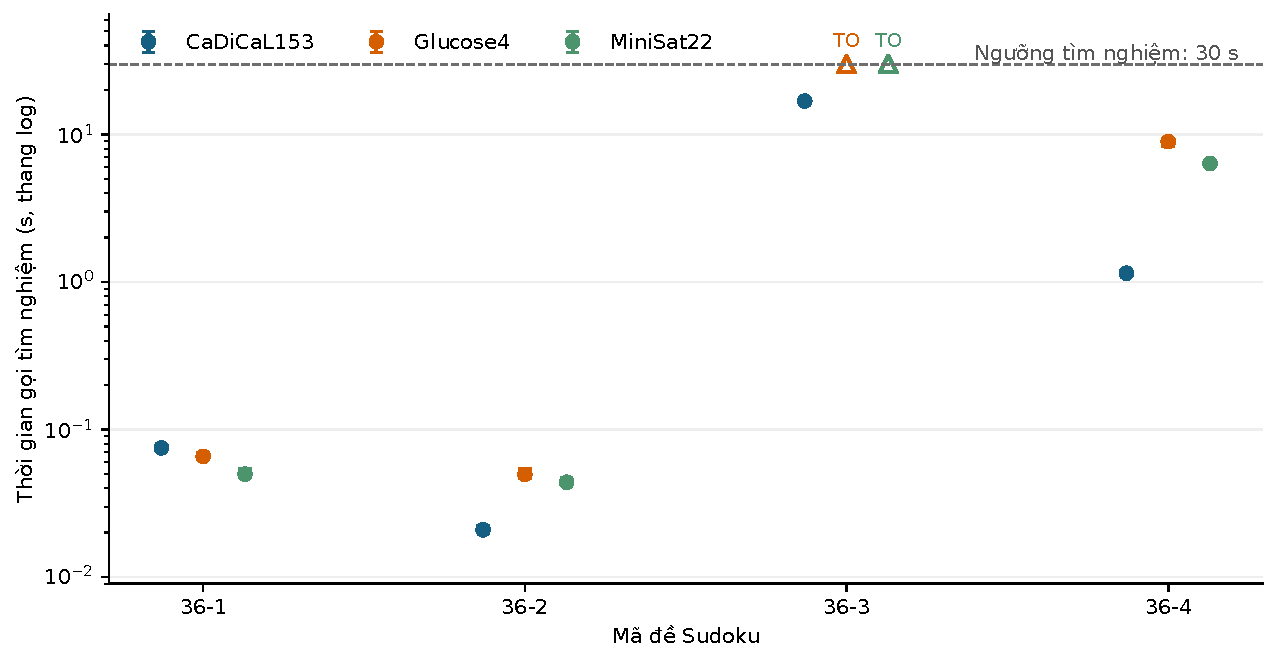
\includegraphics[width=0.92\linewidth]{hinh_phan4/sat_36x36.pdf}
 \caption{Thời gian gọi tìm nghiệm với sequential counter trên bốn đề
 $36\times36$. Trục tung dùng thang log; TO biểu thị timeout cả ba lần.}
 \label{fig:exp-sat36}
\end{figure}

Trên đề $36$-$3$, CaDiCaL153 có thời gian gọi tìm nghiệm trung bình
$16.835$ giây, độ lệch chuẩn mẫu $0.452$ giây; tổng thời gian là
$19.023$ giây. Glucose4 và MiniSat22 hết ngưỡng ở cả ba lượt, với thời
gian gọi giải được ghi xấp xỉ $30$ giây. Tổng thời gian trung bình của
các lượt bị dừng lần lượt là $32.064$ và $32.214$ giây, phù hợp với
việc tổng thời gian còn tính những bước nằm ngoài ngưỡng tìm nghiệm.

Đề $36$-$4$ có ít ô cho trước hơn đề $36$-$3$, nhưng cả ba backend đều
giải được. CaDiCaL153 cần trung bình $1.146$ giây ở lời gọi tìm nghiệm,
trong khi Glucose4 và MiniSat22 lần lượt cần $8.949$ và $6.351$ giây.
Quan sát này cho thấy chỉ đếm ô cho trước không đủ để dự đoán độ khó
đối với SAT; cấu trúc ràng buộc và cách bộ giải khai thác nó cũng ảnh
hưởng đến kết quả.

\begin{table}[pos=htbp]
 \centering
 \caption{Trung bình trên cùng 15 đề được cả ba backend giải thành công, mỗi backend có 45 lượt. Đề $36$-$3$ bị loại khỏi bảng này cho cả ba backend.}
 \label{tab:exp-sat-common}
 \begin{tabular}{lrr}
  \toprule
  Backend & Gọi tìm nghiệm (ms) & Tổng thời gian (s) \\
  \midrule
  CaDiCaL153 & $105.481$ & $0.9004$ \\
  Glucose4 & $624.070$ & $1.3670$ \\
  MiniSat22 & $436.364$ & $1.1790$ \\
  \bottomrule
 \end{tabular}
\end{table}

Trên phần giao $15$ đề giải được bởi cả ba backend, CaDiCaL153 có
trung bình thời gian gọi giải và tổng thời gian thấp nhất
(Bảng~\ref{tab:exp-sat-common}). Đây là nhận xét trên tập dữ liệu đã
khảo sát, không phải khẳng định backend này nhanh nhất trên từng đề.
Ví dụ, trên đề $25$-$3$, MiniSat22 có thời gian gọi tìm nghiệm trung
bình khoảng $0.044$ giây, thấp hơn CaDiCaL153 ở khoảng $0.225$ giây.

\subsection{Ảnh hưởng của mã hóa AMO}

Thí nghiệm này cố định Glucose4 và bốn đề $25\times25$ nhằm tách ảnh
hưởng của mã hóa khỏi lựa chọn backend và kích thước bàn cờ. Cả $60$
quan sát đều trả SAT và có lời giải hợp lệ. Các phương pháp có cùng
$25^3=15\,625$ biến gốc, nhưng khác số biến phụ và số mệnh đề.

\begin{table}[pos=htbp]
 \centering
 \caption{Kích thước và thời gian của năm mã hóa trên bốn đề $25\times25$, Glucose4, ba lượt mỗi đề. Các thời gian là trung bình của 12 lượt; cột mệnh đề chưa cộng $g$.}
 \label{tab:exp-encoding}
 \begin{tabular}{lrrrrr}
  \toprule
  Mã hóa & Biến & Mệnh đề & Sinh CNF (s) & Gọi SAT (ms) & Tổng (s) \\
  \midrule
  pairwise & $15\,625$ & $752\,500$ & $0.5861$ & $21.938$ & $2.4971$ \\
  seqcounter & $75\,625$ & $180\,000$ & $0.1633$ & $70.473$ & $0.8129$ \\
  binary & $28\,125$ & $315\,000$ & $0.2780$ & $10.814$ & $1.1585$ \\
  commander & $45\,625$ & $207\,500$ & $0.3264$ & $16.822$ & $1.0007$ \\
  product & $40\,625$ & $177\,500$ & $0.1764$ & $30.438$ & $0.7740$ \\
  \bottomrule
 \end{tabular}
\end{table}

Bảng~\ref{tab:exp-encoding} ghi số mệnh đề quy tắc trước khi cộng các
ô cho trước; mỗi đề thêm $g$ mệnh đề đơn như
\eqref{eq:method-clause-count}. Ví dụ, pairwise có $752\,500$ mệnh đề
quy tắc, sequential counter có $180\,000$, còn product có $177\,500$.
So với pairwise, product giảm khoảng $76.4\%$ số mệnh đề quy tắc nhưng
tăng số biến do sử dụng biến phụ.

\begin{figure}[pos=htbp]
 \centering
 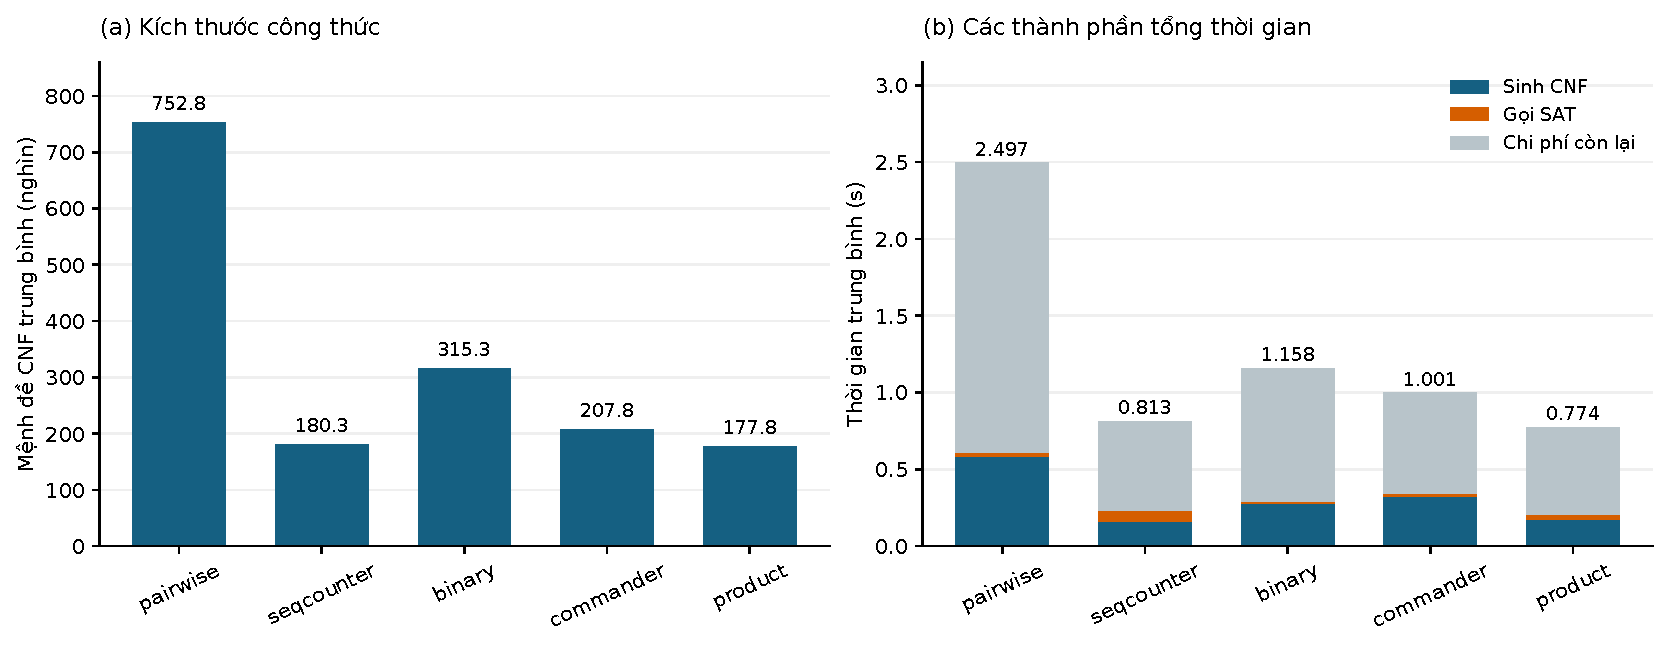
\includegraphics[width=\linewidth]{hinh_phan4/encoding_25x25.pdf}
 \caption{So sánh năm mã hóa trên bốn đề $25\times25$ với Glucose4.
 (a) Số mệnh đề trung bình, gồm cả các ô cho trước.
 (b) Phân rã tổng thời gian trung bình thành sinh CNF, gọi SAT và phần còn lại.}
 \label{fig:exp-encoding}
\end{figure}

Product có tổng thời gian trung bình thấp nhất, khoảng $0.774$ giây,
tiếp theo là sequential counter ở $0.813$ giây. Pairwise cần khoảng
$2.497$ giây, xấp xỉ $3.23$ lần product trong quy trình triển khai này.
Hình~\ref{fig:exp-encoding} cho thấy chênh lệch không chỉ nằm ở thời
gian gọi SAT: sinh CNF và các bước ngoài hai bộ đếm cũng đóng góp đáng
kể. Phần còn lại được tính bằng hiệu của tổng thời gian với thời gian
sinh CNF và gọi SAT, không phải phép đo riêng từng bước truyền dữ liệu.

Binary có thời gian gọi SAT trung bình thấp nhất, khoảng $10.814$ ms,
nhưng tổng thời gian $1.158$ giây vẫn cao hơn product và sequential
counter. Ngược lại, sequential counter có thời gian sinh CNF thấp nhất
trong năm phương pháp ở tập này. Vì vậy, ít mệnh đề hơn, sinh CNF nhanh
hơn và tìm nghiệm nhanh hơn là những tiêu chí cần được xem xét riêng.

Chênh lệch trung bình tổng thời gian giữa product và sequential counter
chỉ khoảng $4.8\%$; product cũng không thấp nhất ở mọi đề. Trên đề
$25$-$4$, sequential counter đạt khoảng $0.801$ giây, trong khi product
là $0.846$ giây. Với bốn đề và ba lần lặp mỗi cấu hình, bài chỉ đưa ra
thống kê mô tả, chưa kết luận khác biệt nhỏ này có ý nghĩa thống kê
hoặc sẽ giữ nguyên trên những bộ dữ liệu khác.

\subsection{Đối chiếu với CP-SAT, CP Optimizer và MIP}

\subsubsection{So sánh trên các đề Sudoku chuẩn}

Bốn đề $9\times9$ là miền dữ liệu chung mà cả bảy cấu hình đều có
đủ ba lượt giải thành công. Bảng~\ref{tab:exp-cross9} tổng hợp $12$
lượt của mỗi cấu hình. Tất cả lời giải trong bảng đều qua cùng hàm
kiểm tra, nhưng số biến và cách diễn đạt ràng buộc đầu vào của các
phương pháp khác nhau.

\begin{table}[pos=htbp]
 \centering
 \caption{Trung bình trên bốn đề $9\times9$, 12 lượt SAT hợp lệ cho mỗi cấu hình. Đơn vị thời gian: ms. Cột tạo mô hình là sinh CNF đối với SAT; phạm vi lời gọi giải khác nhau giữa các API.}
 \label{tab:exp-cross9}
 \begin{tabular}{lrrr}
  \toprule
  Cấu hình & Tạo mô hình & Gọi giải & Tổng thời gian \\
  \midrule
  CaDiCaL153 & $16.678$ & $0.223$ & $182.303$ \\
  Glucose4 & $13.351$ & $0.935$ & $173.813$ \\
  MiniSat22 & $14.675$ & $0.900$ & $179.138$ \\
  CP-SAT & $1.420$ & $5.714$ & $7.380$ \\
  CP Optimizer & $1.009$ & $23.061$ & $24.475$ \\
  CPLEX MIP & $17.339$ & $4.139$ & $22.077$ \\
  Gurobi & $5.197$ & $1.781$ & $8.468$ \\
  \bottomrule
 \end{tabular}
\end{table}

Trên các đề này, CP-SAT và Gurobi có tổng thời gian triển khai trung
bình lần lượt khoảng $7.38$ và $8.47$ ms; CPLEX MIP và CP Optimizer
lần lượt khoảng $22.08$ và $24.48$ ms. Ba cấu hình SAT có tổng thời
gian lớn hơn, dù thời gian gọi tìm nghiệm của CaDiCaL153 rất nhỏ.
Hình~\ref{fig:exp-cross9} biểu diễn cả trung bình theo đề và trung
bình chung, giúp quan sát mức chênh lệch trên cùng bốn đầu vào.

\begin{figure}[pos=htbp]
 \centering
 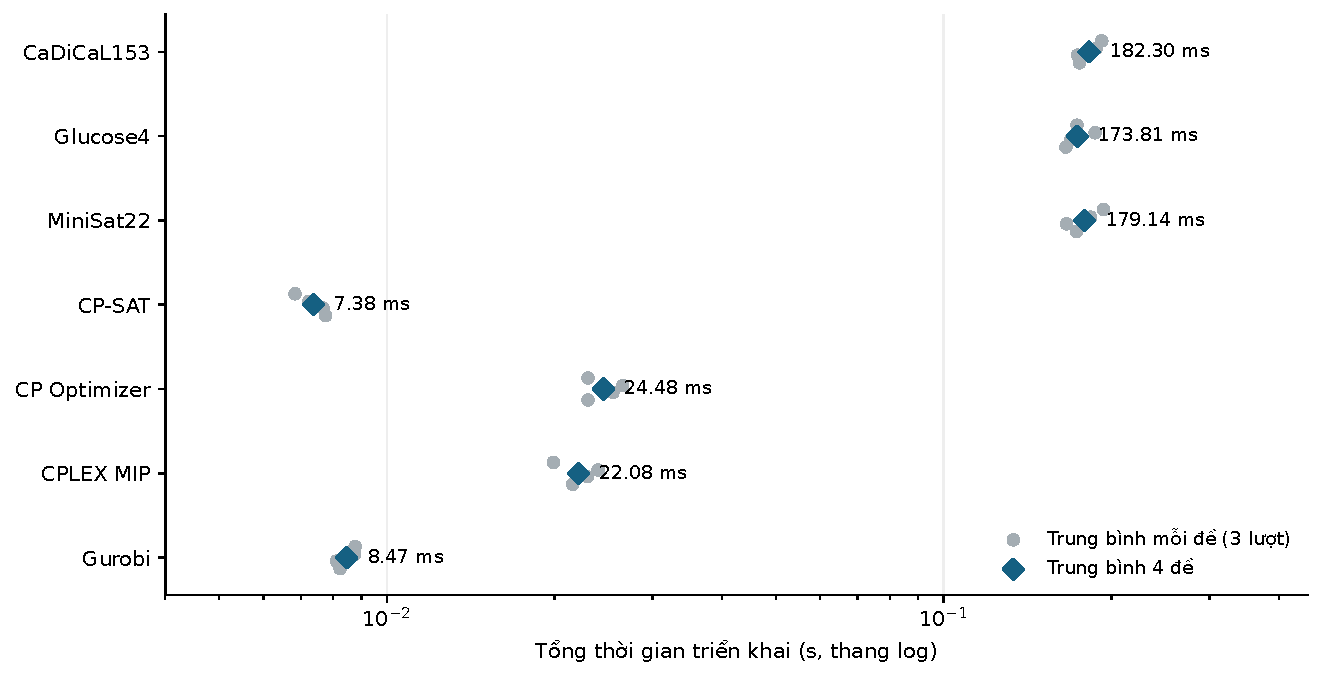
\includegraphics[width=0.94\linewidth]{hinh_phan4/doi_chieu_9x9.pdf}
 \caption{Tổng thời gian triển khai trên cùng bốn đề $9\times9$.
 Mỗi chấm xám là trung bình ba lượt của một đề; hình thoi là trung bình
 bốn đề. Trục thời gian dùng thang log.}
 \label{fig:exp-cross9}
\end{figure}

Kết quả này phản ánh cả mô hình và đường thực thi: SAT có sinh CNF,
ghi DIMACS, khởi tạo tiến trình, nạp công thức và giao tiếp; các API
khác có chi phí xây mô hình và tương tác với engine theo cách riêng.
Do đó, nhận xét phù hợp là quy trình CP-SAT và Gurobi có tổng thời gian
thấp trên tập $9\times9$ hiện tại. Không suy rộng từ bảng này rằng một
họ thuật toán luôn vượt trội họ còn lại trên Sudoku tổng quát.

\subsubsection{Các kích thước lớn và giới hạn môi trường chạy}

CP-SAT giải được cả $16$ đề trong ba lần lặp, tổng cộng $48/48$ lượt
SAT. Trên đề $25$-$3$, tổng thời gian trung bình của CP-SAT khoảng
$0.140$ giây, CaDiCaL153 khoảng $1.063$ giây và CP Optimizer khoảng
$6.905$ giây. Vì vậy mô hình biến nguyên ít biến hơn không tự bảo đảm
thời gian nhỏ hơn trên mọi đầu vào.

\begin{table}[pos=htbp]
 \centering
 \caption{Tổng thời gian trên các đề kích thước lớn (giây). Các giá trị là trung bình ba lượt SAT. LIC: bị giới hạn giấy phép, kèm số lượt đã thử; ---: chưa có bản ghi chạy. CaDiCaL153 dùng sequential counter.}
 \label{tab:exp-large}
 \begin{tabular}{lrrl}
  \toprule
  Mã đề & CaDiCaL153 & CP-SAT & CP Optimizer \\
  \midrule
  16-1 & $0.3117$ & $0.0126$ & $0.0291$ \\
  16-2 & $0.3716$ & $0.0083$ & $0.0314$ \\
  16-3 & $0.3369$ & $0.0344$ & $0.0279$ \\
  16-4 & $0.3109$ & $0.0543$ & $0.0292$ \\
  \addlinespace[3pt]
  25-1 & $0.8590$ & $0.0312$ & $0.0597$ \\
  25-2 & $0.9038$ & $0.0184$ & $0.0372$ \\
  25-3 & $1.0629$ & $0.1400$ & $6.9052$ \\
  25-4 & $0.8908$ & $0.2036$ & LIC (3 lượt) \\
  \addlinespace[3pt]
  36-1 & $2.2445$ & $0.1555$ & LIC (1 lượt) \\
  36-2 & $2.2371$ & $0.0725$ & --- \\
  36-3 & $19.0232$ & $14.7752$ & --- \\
  36-4 & $3.2469$ & $1.1196$ & --- \\
  \bottomrule
 \end{tabular}
\end{table}

Bảng~\ref{tab:exp-large} cho thấy CP-SAT giải được cả bốn đề
$36\times36$, trong đó đề $36$-$3$ cần trung bình $14.775$ giây tổng
thời gian. CaDiCaL153 cũng hoàn thành cả bốn đề; các trường hợp timeout
của Glucose4 và MiniSat22 đã được báo cáo riêng ở phần trước.

CP Optimizer gặp LICENSE\_LIMIT trên cả ba lượt đề $25$-$4$ và một lượt
kiểm tra đề $36$-$1$. Ba đề $36$ còn lại không có bản ghi chạy CP
Optimizer trong tập hiện có, nên được đánh dấu chưa chạy, thay vì gán
một kết quả suy đoán. CPLEX MIP và Gurobi đều bị giới hạn giấy phép ở
lượt kiểm tra đề $16$-$1$; không có dữ liệu hiệu năng thành công của
hai công cụ này cho các kích thước lớn hơn trong bộ thí nghiệm.

Một công cụ từ chối mô hình do giấy phép không có nghĩa bài toán vô
nghiệm, cũng không phải công cụ giải nhanh trong vài chục mili giây.
Giới hạn này làm phạm vi đối chiếu giữa các phương pháp không hoàn
toàn đồng đều; kết luận về CPLEX MIP và Gurobi được giới hạn ở miền
$9\times9$ đã có đủ các lượt giải hợp lệ.

\subsection{Kiểm tra trường hợp vô nghiệm}

Ngoài các đề có nghiệm, hai đầu vào $9\times9$ được dùng để kiểm tra
chức năng phát hiện UNSAT. Cả hai có $31$ ô cho trước.
\texttt{unsat\_duplicate.txt} chứa xung đột lặp số trực tiếp trong một
nhóm; \texttt{unsat\_no\_duplicates.txt} không có lặp số trực tiếp
trên các ô cho trước nhưng vẫn không thể hoàn thành thành Sudoku hợp lệ.

\begin{table}[pos=htbp]
 \centering
 \caption{Kết quả kiểm tra chức năng trên hai đề vô nghiệm. Mỗi ô là kết quả một lượt; SAT dùng Glucose4 và sequential counter.}
 \label{tab:exp-unsat}
 \begin{tabular}{lccccc}
  \toprule
  Đầu vào & SAT & CP-SAT & CP Opt. & CPLEX MIP & Gurobi \\
  \midrule
  Lặp trực tiếp & UNSAT & UNSAT & UNSAT & UNSAT & UNSAT \\
  Không lặp trực tiếp & UNSAT & UNSAT & UNSAT & UNSAT & UNSAT \\
  \bottomrule
 \end{tabular}
\end{table}

Cả năm cấu hình trong Bảng~\ref{tab:exp-unsat} đều kết luận UNSAT
trên hai đầu vào, tương ứng mười lượt kiểm tra chức năng.
SAT trong bảng dùng Glucose4 và sequential counter. Các trường hợp
này được chạy một lượt cho mỗi cặp đề--công cụ, không thuộc thiết kế
ba lần lặp dùng để so sánh thời gian trên $16$ đề có nghiệm.
Trường kiểm tra lời giải được để trống vì không có bảng nghiệm để
đánh giá, không gán một giá trị False như thể đã giải ra bảng sai.

\subsection{Hạn chế và phạm vi diễn giải}

Thứ nhất, mỗi kích thước chỉ có bốn đề. Những đề lớn được tạo từ một
họ bảng cyclic và các phép biến đổi bảo toàn Sudoku; ba đề bổ sung
cùng kích thước dùng mặt nạ lồng nhau. Dữ liệu hữu ích để kiểm tra khả
năng mở rộng của chương trình, nhưng chưa đại diện cho mọi cấu trúc
Sudoku và chưa cho phép suy rộng chắc chắn về độ khó trung bình.

Thứ hai, ba lần lặp chủ yếu giúp quan sát dao động thời gian trên cùng
máy và cấu hình. Thí nghiệm chưa kiểm soát riêng xung nhịp CPU, trạng
thái bộ nhớ đệm hoặc tải nền; thứ tự chạy các cấu hình chưa được ghi
đủ để xác nhận một thiết kế ngẫu nhiên hóa. Bài không thực hiện kiểm
định khác biệt giữa các trung bình. Vì vậy những chênh lệch nhỏ được xem như kết quả mô tả,
không phải bằng chứng thống kê về ưu thế tổng quát.

Thứ ba, giới hạn giấy phép làm miền so sánh thương mại không đầy đủ.
Số ràng buộc CP/MIP cũng không cùng đơn vị với số mệnh đề CNF, và
thời gian gọi giải của các API có ranh giới đo khác nhau.
Các nhật ký SAT chưa lưu riêng cột giới hạn thời gian, hạt giống hoặc
thứ tự chạy; thông tin này cần được giữ cùng lệnh và cấu hình thí
nghiệm để việc tái lập đầy đủ hơn.

Trong phạm vi đã khảo sát, các kết quả hỗ trợ ba nhận xét chính:
CaDiCaL153 hoàn thành toàn bộ bộ đề với sequential counter;
lựa chọn mã hóa có ảnh hưởng lớn đến kích thước CNF và tổng thời gian;
và các mô hình CP-SAT, CP, MIP có thể cho hành vi rất khác nhau tùy
đề, chi phí triển khai và giới hạn môi trường. Các nhận xét này được
đặt trong đúng phạm vi dữ liệu và điều kiện đo nêu trên.

\section{Thảo luận và kết luận}
\label{sec:ketluan}

\subsection{Đánh giá cách tiếp cận SAT}

Các kết quả ở Mục~\ref{sec:thucnghiem} cho thấy hiệu quả của cách tiếp
cận SAT phụ thuộc đồng thời vào biểu diễn ràng buộc, bộ giải và quy
trình thực thi. Số biến gốc $N^3$ được xác định bởi cách biểu diễn một
lựa chọn ô--giá trị, nhưng phần biến phụ và số mệnh đề thay đổi đáng kể
theo mã hóa AMO. Vì vậy, đánh giá một mô hình chỉ qua tổng số biến hoặc
tổng số mệnh đề sẽ bỏ qua những yếu tố quan trọng khác.

Chẳng hạn, sequential counter có nhiều biến hơn pairwise nhưng ít
mệnh đề hơn và tổng thời gian trung bình thấp hơn trong thí nghiệm
mã hóa. Binary có thời gian gọi SAT thấp nhất trên bốn đề
$25\times25$ với Glucose4, trong khi product có tổng thời gian thấp
nhất. Sự khác biệt này cho thấy cần đánh giá riêng chi phí dựng công
thức và chi phí tìm mô hình, sau đó xem xét cả tổng thời gian mà người
dùng thực sự chờ. Một công thức thuận lợi cho tìm nghiệm vẫn có thể
tốn thời gian hơn ở các bước xây dựng, lưu trữ hoặc chuyển vào bộ giải.

Số ô cho trước cũng không xác định đơn độc độ khó của bài toán SAT.
Trong ba đề bổ sung cùng kích thước, việc bỏ thêm số làm các ràng buộc
đề bài yếu đi và tập lời giải có thể lớn hơn. Vì chương trình chỉ cần
tìm một lời giải, sự mở rộng đó có thể làm một số trường hợp dễ giải
hơn, dù đề có ít dữ kiện hơn. Điều này phù hợp với quan sát đề
$36$-$4$ được giải nhanh hơn đề $36$-$3$ ở cả ba backend. Không thể
đồng nhất độ khó tìm một nghiệm bằng SAT với độ khó giải tay hoặc yêu
cầu xác định một nghiệm duy nhất.

Một điểm cần tách biệt là tính đúng đắn của mô hình và hiệu năng bộ
giải. Lập luận hai chiều ở Mục~\ref{sec:phuongphap} xác định sự tương
ứng giữa lời giải Sudoku và mô hình CNF, với giả thiết các mã hóa EO
đúng và biến phụ không trùng nhau. Hàm kiểm tra nghiệm bổ sung một lớp
đối chiếu trực tiếp trên bàn cờ sau giải mã. Các kết quả thực nghiệm
cung cấp bằng chứng về hoạt động của bản cài đặt trên những trường hợp
đã thử; chúng không thay thế lập luận đúng đắn cho mô hình tổng quát.

\subsection{Đóng góp và phạm vi kết quả}

Bài tập xây dựng được một quy trình giải Sudoku tổng quát từ đầu vào
dạng ma trận đến kết quả được kiểm tra và nhật ký thực nghiệm. Quy
trình cấp trước toàn bộ biến gốc bằng một ánh xạ xác định, quản lý biến
phụ dùng chung bộ cấp mã, sinh đầy đủ bốn nhóm quy tắc EO và các mệnh
đề đơn, sau đó giải mã độc lập với thứ tự literal trong mô hình.
Việc tách hàm sinh EO khỏi các nhóm Sudoku giúp sử dụng cùng một mô
hình để khảo sát nhiều cách mã hóa AMO.

Ở cấp độ triển khai, ba mã hóa pairwise, sequential counter và bitwise
được khai thác qua CardEnc; commander nhóm ba và product một tầng
được sinh bằng các hàm riêng. Các bộ chuyển tiếp CP-SAT, CP Optimizer,
CPLEX MIP và Gurobi cung cấp những biểu diễn đối chứng dùng biến nguyên
hoặc biến nhị phân. Đóng góp của bài nằm ở việc xây dựng, giải thích,
kiểm tra và đánh giá các mô hình này trong một quy trình thực nghiệm
có ghi nhận trạng thái và phạm vi đo rõ ràng.

Về độ phủ của thí nghiệm backend, CaDiCaL153 với sequential counter
hoàn thành cả $48/48$ lượt trên $16$ đề, còn Glucose4 và MiniSat22 mỗi
bộ hoàn thành $45/48$ lượt. Trên phần giao $15$ đề đều giải được,
CaDiCaL153 có trung bình tổng thời gian thấp nhất trong ba backend
(Bảng~\ref{tab:exp-sat-common}). Đồng thời, CP-SAT cũng hoàn thành
cả $48/48$ lượt của bộ đề chính. Những kết quả này hỗ trợ đánh giá
khả năng xử lý các đầu vào đã khảo sát, nhưng không thiết lập một thứ
hạng chung cho mọi bài Sudoku.

Thí nghiệm mã hóa chỉ so sánh năm lựa chọn với Glucose4 trên
$25\times25$, trong khi thí nghiệm backend giữ cố định sequential
counter. Vì vậy, không thể ghép hai kết quả riêng để kết luận
CaDiCaL153 kết hợp product là cấu hình tốt nhất trên các kích thước
lớn hơn. Tương tự, dữ liệu MIP bị giới hạn giấy phép ngoài miền
$9\times9$ không cho phép suy ra giới hạn tính toán của phiên bản đầy
đủ. Phạm vi kết luận phải gắn với những tổ hợp cấu hình thực sự đã chạy.

\subsection{Hướng phát triển}

Một hướng tiếp tục là mở rộng bộ dữ liệu và thiết kế thí nghiệm theo
cả ba chiều: kích thước, mã hóa và backend. Cần bổ sung những đề từ
nhiều nguồn hoặc nhiều họ cấu trúc khác nhau, ghi nhận quan hệ giữa
các đề sinh, và phân biệt trường hợp có nghiệm duy nhất với trường hợp
có thể có nhiều nghiệm. Khi so sánh các cấu hình, có thể tăng số lần
lặp, ngẫu nhiên hóa thứ tự chạy và lưu phiên bản mã nguồn cùng tham số
giới hạn, hạt giống và môi trường. Những thay đổi này sẽ làm rõ mức
dao động và phạm vi khái quát của các nhận xét hiệu năng.

Về triển khai, cần đo riêng chi phí ghi DIMACS, khởi tạo tiến trình,
nạp công thức và kiểm tra nghiệm để xác định phần chi phí có thể giảm.
Việc tái sử dụng thành phần CNF quy tắc giữa các đề cùng kích thước
hoặc tái sử dụng tiến trình là những hướng có thể khảo sát. Tuy nhiên,
nếu áp dụng, cần phân biệt lượt khởi tạo mới với lượt dùng lại trạng
thái và đo lại các cấu hình tương ứng, vì ranh giới thời gian sẽ thay
đổi so với các số liệu hiện tại.

Một mở rộng khác là kiểm tra tính duy nhất của lời giải. Giả sử đã
tìm được lời giải $S$. Có thể thêm vào công thức một mệnh đề chặn
\begin{equation}
 C_{\mathrm{block}}(S)=
 \bigvee_{r\in I}\bigvee_{c\in I}\neg x_{r,c,S_{r,c}},
 \label{eq:conclusion-uniqueness}
\end{equation}
để yêu cầu ít nhất một ô khác với $S$. Nếu
$F_e(A)\land C_{\mathrm{block}}(S)$ là SAT thì có một bàn cờ nghiệm
khác; nếu là UNSAT thì $S$ là nghiệm duy nhất của đề đã mã hóa.
Trường hợp chưa kết luận do hết giờ phải được giữ là chưa xác định.
Mệnh đề chặn cần dựa trên các biến gốc, vì hai phép gán khác nhau chỉ
ở biến phụ chưa chắc biểu diễn hai lời giải Sudoku khác nhau. Đây là
hướng mở rộng, chưa phải bước được thực hiện trong các lượt benchmark
của báo cáo.

\subsection{Kết luận}

Bài tập đã mô hình hóa Sudoku tổng quát bằng SAT với ánh xạ biến và
các nhóm ràng buộc được trình bày tường minh, đồng thời triển khai
quy trình giải bằng PySAT, kiểm tra nghiệm và ghi nhận thống kê.
Thực nghiệm trên các kích thước từ $9\times9$ đến $36\times36$ cho
thấy cách tiếp cận xử lý được bộ dữ liệu đã chọn và phân biệt được
trường hợp có nghiệm, vô nghiệm, hết thời gian và giới hạn môi trường.

Kết quả so sánh cho thấy lựa chọn mã hóa ảnh hưởng đến cả kích thước
công thức lẫn tổng thời gian. Trên bốn đề $25\times25$ với Glucose4,
product và sequential counter có tổng thời gian trung bình thấp hơn
pairwise; binary lại có thời gian gọi SAT trung bình thấp nhất.
CaDiCaL153 với sequential counter có độ phủ thành công đầy đủ trong
thí nghiệm backend, trong khi đối chiếu CP-SAT và các công cụ CP/MIP
cho thấy cần đánh giá cả chi phí triển khai và điều kiện chạy.

Qua đó, bài tập cung cấp một cơ sở cài đặt và thực nghiệm để tiếp tục
khảo sát việc giải Sudoku bằng SAT. Kết luận được giới hạn ở bộ đề,
cấu hình và cách đo đã công bố; việc mở rộng dữ liệu, hoàn thiện khả
năng tái lập và khảo sát thêm các tổ hợp mã hóa--backend là những bước
tiếp theo để có đánh giá đầy đủ hơn.

\section*{Mã nguồn và dữ liệu}
\url{https://github.com/dungbui1326/sudoku-sat-btl1}


\end{document}
